\chapter{Nonlinear manifold projection-based reduced order models}
\label{chap:nonlinear_prom}

%Alternative
While linear reduced-order models have proven effective in a range of problems with smooth and low-dimensional solution manifolds, they face critical limitations in regimes dominated by transport phenomena, shock formation, and nonlinear interactions. As seen in the parametric one-dimensional Burgers' problem studied previously, even the most robust linear projections, such as LSPG, struggle to achieve accurate approximations without requiring a prohibitively large number of modes. This behavior reflects the well-known limitations imposed by the Kolmogorov $n$-width barrier~\cite{Quarteroni2014, pinkus2012n}, which restricts the compressibility of the solution manifold and ultimately the efficiency of any linear approximation.

To overcome this bottleneck, nonlinear PMOR has emerged as a powerful alternative. This broader class of methods has demonstrated strong potential in various applications, including structural dynamics~\cite{he2020situ}, compressible and hypersonic CFD~\cite{chmiel2025unified}, and turbulent wake flows~\cite{barnett2022quadratic}, among others.

A diverse set of nonlinear PMOR strategies has been proposed in the literature. Piecewise-affine approximations~\cite{amsallem2012nonlinear, grimberg2021mesh} exploit local linearity and have shown real-time performance in RANS simulations and LES-based fighter jet models. Registration-based techniques~\cite{taddei2020registration, mirhoseini2022model} offer a powerful framework for transport-dominated problems, introducing mesh motion to align dominant features across parameter configurations. Quadratic approximation manifolds~\cite{jain2017quadratic, barnett2022quadratic} offer a simulation-free or data-driven approach with demonstrable improvements in both accuracy and efficiency. Additionally, convolutional autoencoder-based models~\cite{lee2020model, romor2023non} leverage deep neural architectures to learn structured, low-dimensional manifolds directly from high-dimensional flow data, enabling expressive yet compact representations for complex nonlinear dynamics. While these deep learning-based methods effectively address the Kolmogorov $n$-width barrier, their scalability to full-scale industrial problems, particularly those involving high-resolution meshes with millions of degrees of freedom, remains limited and largely untested. This challenge has motivated hybrid strategies such as POD-DL-ROM~\cite{FRESCA2022114181}, which combine POD-based compression with neural decoders to mitigate computational overhead while retaining nonlinear expressivity.


A particularly promising direction is the intrusive latent-space closure modeling framework introduced in~\cite{barnett2023neural} and mathematically analyzed in~\cite{cohen2023nonlinear}, which augments the classical affine approximation by modeling its closure error using a nonlinear map in latent space. This methodology, implemented via PROM-ANN, has demonstrated state-of-the-art performance in large-scale CFD applications, including problems with millions of degrees of freedom, delivering online acceleration by up to three orders of magnitude while maintaining high accuracy, even at reduced dimensions as low as $n = 2$~\cite{chmiel2025unified}. However, these deep learning approaches often suffer from non-interpretability and require substantial training data, which limits their theoretical grounding and practical usability in data-scarce regimes.

To address these challenges, this thesis contributes to recent advances in interpretable, data-efficient, and physics-consistent nonlinear map constructions for reduced-order modeling. In particular, it explores two complementary research directions that target the limitations of nonlinear latent-space closure models: first, the introduction of a discrete physics-informed training strategy for PROM-ANN~\cite{sibuet2025discrete}, which augments standard snapshot-based training with a residual-based loss derived from the underlying finite element formulation; and second, the development of interpretable kernel-based latent-space closure models, namely PROM-GPR and PROM-RBF~\cite{de2025nonlinear}, which replace the neural network with Gaussian process regression (GPR) or radial basis function (RBF) interpolation. Both strategies preserve the latent-space correction structure while enhancing either the physical consistency or the theoretical interpretability of the resulting manifold PROMs.

This chapter does not develop these extensions in full; instead, it serves as a unified conceptual and methodological survey that establishes the context for these advancements. By reviewing the progression from global linear subspace approximations to more expressive nonlinear manifold formulations, culminating in latent-space closure modeling, this chapter situates the motivation for the methodological improvements and alternatives presented in the subsequent chapters. In doing so, it clarifies how overcoming the Kolmogorov $n$-width barrier through nonlinear manifold constructions can significantly improve the efficiency of reduced-order models, and why exploring the incorporation of physical insight into the training process may offer additional benefits in terms of stability, interpretability, or generalization.

A comprehensive formulation, implementation, and validation of the discrete physics-informed training for PROM-ANN is presented in Chapter~\ref{chap:article3}, while the PROM-GPR and PROM-RBF approaches are developed and analyzed in depth in Chapter~\ref{chap:article4}. The remainder of this chapter therefore focuses on situating these contributions within the broader landscape of nonlinear PMOR, using the one-dimensional Burgers' problem as a representative test case to illustrate the strengths and limitations of different manifold-based strategies.




\section{Minimum-residual projection on nonlinear manifolds}
\label{subsec:minres-manifold-rom}

Let us recall the fully discrete set of governing equations derived in the previous chapters, written in terms of a residual operator \( \mathbf{R}: \mathbb{R}^{N} \times [0, T] \times \mathcal{D} \rightarrow \mathbb{R}^{N} \), as
\begin{equation}
\mathbf{R}(\mathbf{u}(t, \boldsymbol{\mu}); t, \boldsymbol{\mu}) = \mathbf{0},
\label{eq:residual_discrete_manifold}
\end{equation}
where \( \mathbf{u}(t, \boldsymbol{\mu}) \in \mathbb{R}^{N} \) denotes the high-fidelity solution at time \( t \in [0, T] \) and for parameter configuration \( \boldsymbol{\mu} \in \mathcal{D} \subset \mathbb{R}^p \).

As discussed in Chapter~\ref{chap:article1}, solving this high-dimensional nonlinear system at each time step and for each parameter configuration can be computationally expensive. 
There, the solution $\mathbf{u}(t,\boldsymbol{\mu})$ was approximated using a linear subspace projection, and the corresponding residual was minimized in a weighted norm. 
To extend this strategy, a general approximation manifold is now considered by expressing the solution through a general decoder function:
\begin{equation}
\mathbf{u}(t,\boldsymbol{\mu}) \;\approx\; \mathbf{\tilde{u}}(t,\boldsymbol{\mu}) 
= \mathbf{u}_{\text{ref}} + D_u(\mathbf{q}(t,\boldsymbol{\mu})),
\label{eq:general_decoder}
\end{equation}
where $\mathbf{u}_{\text{ref}} \in \mathbb{R}^N$ is a chosen reference state, 
$D_u : \mathbb{R}^{n} \rightarrow \mathbb{R}^{N}$ is a general decoder, 
and $\mathbf{q}(t,\boldsymbol{\mu}) \in \mathbb{R}^{n}$ denotes the reduced generalized coordinates. 
An encoder $E_u : \mathbb{R}^{N} \rightarrow \mathbb{R}^{n}$ may also be defined, satisfying $\mathbf{q}(t,\boldsymbol{\mu}) = E_u(\mathbf{u}(t,\boldsymbol{\mu}))$. 
In the linear PROM of Chapter~\ref{chap:linear_prom}, this general formulation reduces to the affine approximation 
$\tilde{\mathbf{u}} = \mathbf{u}_{\text{ref}} + \boldsymbol{\Phi}\mathbf{q}$, which in practice is taken with $\mathbf{u}_{\text{ref}}=0$, 
so that $D_u(\mathbf{q}) = \boldsymbol{\Phi}\mathbf{q}$ and the encoder corresponds to the orthogonal projection $E_u(\mathbf{u}) = \boldsymbol{\Phi}^T \mathbf{u}$. 
For notational simplicity, the following derivations will assume $\mathbf{u}_{\text{ref}}=0$.

The nonlinear encoder–decoder structure associated with this general manifold approximation is illustrated in Figure~\ref{fig:nonlinear_manifold_encoder_decoder}.
\begin{figure}[ht!]
    \centering
    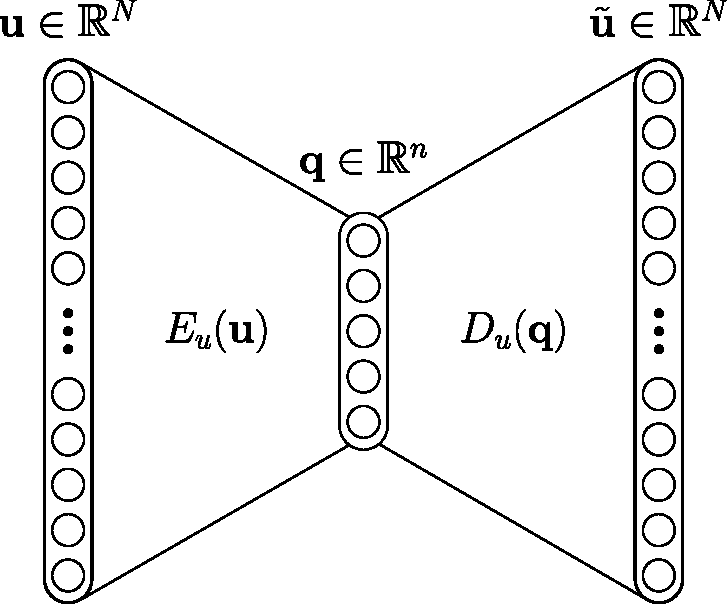
\includegraphics[width=0.5\textwidth]{Figures/nonlinear_manifold_encoder_decoder.pdf}
    \caption{
    Schematic representation of the nonlinear manifold reduction and reconstruction process.
    The high-dimensional state \( \mathbf{u} \in \mathbb{R}^{N} \) is encoded as latent coordinates \( \mathbf{q} \in \mathbb{R}^{n} \) via a nonlinear encoder \( E_u(\mathbf{u}) \), 
    and the approximation \( \tilde{\mathbf{u}} = D_u(\mathbf{q}) \) is reconstructed through a nonlinear decoder \( D_u \). 
    The linear PROM of Chapter~\ref{chap:linear_prom} is recovered as the special case \(D_u(\mathbf{q})=\boldsymbol{\Phi}\mathbf{q}\) with encoder \(E_u(\mathbf{u})=\boldsymbol{\Phi}^T\mathbf{u}\).
    }
    \label{fig:nonlinear_manifold_encoder_decoder}
\end{figure}

Substituting \eqref{eq:general_decoder} into the residual \eqref{eq:residual_discrete_manifold} (with $\mathbf{u}_{\text{ref}}=0$ for simplicity) yields a residual defined on the general approximation manifold:
\begin{equation}
\mathbf{R}(D_u(\mathbf{q}(t, \boldsymbol{\mu}));\,t,\boldsymbol{\mu}).
\end{equation}



Following the residual minimization formulation established for linear subspace PROMs in Chapters~\ref{chap:linear_prom} and ~\ref{chap:article1}, the projection problem is generalized to arbitrary decoders by solving
\begin{equation}
\min_{\mathbf{q}(t, \boldsymbol{\mu}) \in \mathbb{R}^{n}} 
\; \frac{1}{2} \left\lVert 
\mathbf{R}(D_u(\mathbf{q}(t, \boldsymbol{\mu})); t, \boldsymbol{\mu}) 
\right\rVert_{\mathbf{G}}^2,
\label{eq:nonlinear_projection_minimization}
\end{equation}
where \( \|\cdot\|_{\mathbf{G}} \) denotes a norm induced by a symmetric positive definite (SPD) matrix \( \mathbf{G} \in \mathbb{R}^{N \times N} \) (i.e. \( \|\mathbf{v}\|_{\mathbf{G}}^{2} := \mathbf{v}^{T}\mathbf{G}\mathbf{v} \)). This minimization problem extends the optimality conditions from linear PROMs to general approximation manifolds.

\textbf{Notation.} To avoid cumbersome expressions, explicit dependences on \(t\), \(\boldsymbol{\mu}\), and \(\mathbf{q}\) will be omitted after the next equations; unless stated otherwise, all quantities should be understood as functions of \(t\), \(\boldsymbol{\mu}\), and the current reduced state. These dependencies may be reintroduced later in the chapter where appropriate.

The first-order optimality condition associated with \eqref{eq:nonlinear_projection_minimization} leads to the nonlinear system:
\begin{equation}
\left[
\frac{\partial \mathbf{R}}{\partial \mathbf{u}} 
\frac{\partial D_u}{\partial \mathbf{q}}
\right]^T
\mathbf{G} \, 
\mathbf{R} = \mathbf{0},
\end{equation}
which can be expressed in terms of the Jacobian of the residual as:
\begin{equation}
\left[
\mathbf{J} 
\frac{\partial D_u}{\partial \mathbf{q}}
\right]^T
\mathbf{G} \, 
\mathbf{R} = \mathbf{0},
\end{equation}
where \( \mathbf{J} := \tfrac{\partial \mathbf{R}}{\partial \mathbf{u}} \in \mathbb{R}^{N \times N} \).

This projected residual admits an interpretation as a generalized encoder of the residual:
\begin{equation}
E_r(\mathbf{R}) := 
\left(\frac{\partial D_u}{\partial \mathbf{q}}\right)^T 
\mathbf{J}^T 
\mathbf{G} \, \mathbf{R},
\label{eq:general_residual_encoder}
\end{equation}
yielding the reduced residual equation:
\begin{equation}
\mathbf{r}(\mathbf{q}) := E_r\left(\mathbf{R}\right) = \mathbf{0}.
\end{equation}


This nonlinear system in reduced coordinates is solved using a Newton-type iteration:
\begin{equation}
\frac{\partial \mathbf{r}}{\partial \mathbf{q}}^{(k)} \, \delta \mathbf{q}^{(k)} = -\,\mathbf{r}^{(k)},
\end{equation}
which expands to:
\begin{equation}
\left(
\frac{\partial D_u}{\partial \mathbf{q}}
\right)^{(k)T}
\!\!\mathbf{J}^T 
\mathbf{G} 
\mathbf{J}
\left(
\frac{\partial D_u}{\partial \mathbf{q}}
\right)^{(k)} \delta \mathbf{q}^{(k)}
= -
\left(
\frac{\partial D_u}{\partial \mathbf{q}}
\right)^{(k) T}
\!\!\mathbf{J}^T 
\mathbf{G} 
\mathbf{R}^{(k)}.
\label{eq:general_manifold_update}
\end{equation}



Equation~\eqref{eq:general_manifold_update} defines the reduced-order model on a general approximation manifold specified by the decoder \( D_u \), and generalizes the minimum-residual projection framework developed in Chapters~\ref{chap:linear_prom} and ~\ref{chap:article1}. A detailed derivation of this reduced system, including the assumptions involved in the Newton approximation, is provided in Appendix~\ref{app:gauss_newton_manifold}.

\paragraph{Galerkin projection.} 
The Galerkin projection is particularly effective when the Jacobian \( \mathbf{J} \) is SPD. In such cases, setting \( \mathbf{G} = \mathbf{J}^{-T} \) in the minimum-residual condition yields optimal search directions. Substituting this choice into the reduced system \eqref{eq:general_manifold_update} leads to the Galerkin form:
\begin{equation}
\left( \frac{\partial D_u}{\partial \mathbf{q}} \right)^T 
\mathbf{J} 
\left( \frac{\partial D_u}{\partial \mathbf{q}} \right) \delta \mathbf{q} 
= - \left( \frac{\partial D_u}{\partial \mathbf{q}} \right)^T \mathbf{R}.
\label{eq:prom_general_galerkin}
\end{equation}

\paragraph{Least-Squares Petrov–Galerkin (LSPG) projection.} 
In nonlinear problems, the Jacobian \( \mathbf{J} \) is generally not SPD. To address this, the LSPG method adopts \( \mathbf{G} = \mathbf{I} \), ensuring that the reduced model retains the minimum-residual property, which is essential for accuracy and stability. The resulting system becomes:
\begin{equation}
\left( \frac{\partial D_u}{\partial \mathbf{q}} \right)^T 
\mathbf{J}^T 
\mathbf{J} 
\left( \frac{\partial D_u}{\partial \mathbf{q}} \right) \delta \mathbf{q} 
= - \left( \frac{\partial D_u}{\partial \mathbf{q}} \right)^T \mathbf{J}^T \mathbf{R}.
\label{eq:prom_general_lspg}
\end{equation}

\paragraph{}
The preceding formulation establishes a unified framework for projection-based ROMs on general approximation manifolds, encompassing both the Galerkin and LSPG variants as particular cases defined by the choice of the weighting matrix \( \mathbf{G} \). For the remainder of this chapter, the LSPG formulation will be adopted as the standard projection strategy, owing to its improved robustness in convection-dominated systems.

As previously shown in Section~\ref{subsec:galerkin_lspg_comparison}, the one-dimensional inviscid Burgers’ equation was used to illustrate the shortcomings of Galerkin projection in convection-dominated regimes and the stabilizing effect of LSPG. That section also examined key factors such as the construction of the POD basis, the decay of singular values, and the influence of the Kolmogorov \( n \)-width on linear ROM performance.

These findings now serve as a starting point for exploring strategies to overcome the limitations of linear subspace models. Using the same Burgers model problem as a representative testbed, the following sections examine nonlinear ROMs defined on expressive approximation manifolds, aiming to mitigate the Kolmogorov barrier and improve representational accuracy under strong nonlinearity.

\section{Piecewise-linear manifolds via local POD}
The linear subspace approximation underlying classical projection-based ROMs, as discussed in Chapter~\ref{chap:linear_prom}, relies on constructing a global basis \( \boldsymbol{\Phi} \in \mathbb{R}^{N \times n} \) that optimally captures the solution manifold in the least-squares sense. While this approach is effective for smooth or weakly nonlinear problems, it faces severe limitations in transport-dominated regimes (such as the one-dimensional inviscid Burgers' equation examined earlier). In that case, achieving acceptable accuracy required a large number of global modes \( n \), reflecting a large Kolmogorov \( n \)-width and the inability of a single global linear subspace to capture sharp gradients and localized features across the parameter domain and time.

One natural strategy to mitigate this limitation is to abandon the idea of a single global basis and instead adopt \emph{local linear approximations}. This is the principle behind piecewise-linear manifolds and Local POD methods~\cite{amsallem2012nonlinear, grimberg2021mesh}, which partition the solution space into regions where local bases provide more accurate and compact representations. By constructing multiple local bases \( \{ \boldsymbol{\Phi}_i \} \), each tailored to a specific region of the trajectory or parameter space, these methods can better resolve complex solution features with fewer modes per local basis. This local structure effectively lowers the approximation barrier imposed by the global Kolmogorov \( n \)-width and leads to more efficient reduced-order models.

Beyond their conceptual simplicity, piecewise-linear approaches have demonstrated remarkable success in large-scale applications such as transonic aerodynamics and unsteady turbulent flows~\cite{washabaugh2016use, grimberg2021mesh}, delivering real-time or near-real-time performance even in high-dimensional problems with \( N > 10^7 \) degrees of freedom. In the context of the Burgers' model problem considered here, they provide an ideal test case to illustrate how localized bases can significantly improve approximation accuracy.

\subsection{Local subspace construction, clustering, and online basis selection}

To overcome the inherent limitations of global linear subspaces, local POD partitions the solution manifold into smaller regions, each characterized by its own local linear basis tailored specifically to the dynamics of that region.

 The construction described in the following paragraphs, based on clustering in a reduced coordinate space and local POD basis generation, is not unique and does not represent the main methodological contribution of this thesis. It is provided here as a representative formulation to illustrate the key steps involved in building piecewise-linear manifold approximations. A version of this approach was employed in the collaborative work~\cite{bravo2024subspace}.


The local approximation at each time $t$ and parameter configuration $\boldsymbol{\mu}$ is expressed as:
\begin{equation}
\mathbf{u}(t,\boldsymbol{\mu}) \approx \mathbf{\tilde{u}}(t,\boldsymbol{\mu}) 
= \mathbf{u}_{\text{ref},c} + \boldsymbol{\Phi}_c \, \mathbf{q}_c(t,\boldsymbol{\mu}), 
\quad c = 1, \dotsc, N_{\text{local}},
\label{eq:local_pod_approximation}
\end{equation}
where $\mathbf{u}_{\text{ref},c} \in \mathbb{R}^{N}$ denotes the reference state for cluster $c$, 
$\boldsymbol{\Phi}_c \in \mathbb{R}^{N\times n_c}$ is the local POD basis of cluster $c$, 
and $\mathbf{q}_c(t,\boldsymbol{\mu}) \in \mathbb{R}^{n_c}$ are the corresponding local reduced coordinates. 
For notational simplicity, the following derivations will assume $\mathbf{u}_{\text{ref},c}=0$.




\paragraph{Global basis and clustering strategy} 
A global basis \(\boldsymbol{\Phi}_{g}\) is initially constructed by applying POD (via SVD) to the entire snapshot set \(\mathbf{S}\in\mathbb{R}^{N\times N_s}\):
\begin{equation}
\mathbf{S} = \boldsymbol{\Phi}_{g}\,\boldsymbol{\Sigma}_{g}\,\mathbf{V}_{g}^T,
\label{eq:global_svd}
\end{equation}
where \(\boldsymbol{\Phi}_{g}\in\mathbb{R}^{N\times n_g}\) contains the first \(n_g\) global POD modes retained based on a prescribed energy tolerance.

The snapshots are projected onto this global basis to obtain a lower-dimensional representation:
\begin{equation}
\mathbf{q}_{g} = \boldsymbol{\Phi}_{g}^T\,\mathbf{S}\in\mathbb{R}^{n_g\times N_s}.
\label{eq:global_projection}
\end{equation}
A clustering algorithm such as k-means is then applied in this reduced-dimensional coordinate space, partitioning the snapshots into \(N_{\text{local}}\) distinct clusters~\cite{amsallem2012nonlinear, hastie2009elements}. This partitioning yields submatrices \(\mathbf{S}_c\) that contain snapshots assigned to each local cluster:
\begin{equation}
\mathbf{S} = [\mathbf{S}_1,\mathbf{S}_2,\dotsc,\mathbf{S}_{N_{\text{local}}}],
\quad \mathbf{S}_c \in \mathbb{R}^{N \times {N_s}_{(c)}},
\label{eq:local_snapshot_partition}
\end{equation}
where \({N_s}_{(c)}\) is the number of snapshots within the cluster \(c\).

\paragraph{Local basis construction}
For each local snapshot subset \(\mathbf{S}_c\), a local POD basis is computed via SVD:
\begin{equation}
\mathbf{S}_c = \boldsymbol{\Phi}_c \, \boldsymbol{\Sigma}_c \, \mathbf{V}_c^T,
\label{eq:local_svd}
\end{equation}
where \(\boldsymbol{\Phi}_c\in\mathbb{R}^{N\times n_c}\) contains the left singular vectors representing local modes. The local basis dimension \(n_c\) is chosen based on a POD energy criterion:
\begin{equation}
\epsilon(n_c) = 1 - \frac{\sum_{i=1}^{n_c}\sigma_{k,i}^{2}}{\sum_{j=1}^{r_c}\sigma_{k,j}^{2}} \leq \epsilon_{\text{tol}},
\label{eq:local_pod_energy}
\end{equation}
with singular values \(\sigma_{k,i}\) ordered in descending magnitude, and \(r_c\) the numerical rank of cluster \(c\).

\paragraph{Overlapping clusters for smooth transitions}
To ensure smooth transitions between neighboring local subspaces, snapshots near cluster boundaries are included in multiple clusters. A threshold distance criterion in the global reduced space defines the overlap~\cite{Washabaugh2012}. Specifically, snapshots satisfying
\[
\|\mathbf{q}_{g,i} - \mathbf{c}_c\|_2 < \delta_{\text{overlap}},
\]
where \(\mathbf{c}_c\) is the centroid of cluster \(c\), are assigned simultaneously to multiple clusters. The overlapping snapshots between clusters \(c\) and \(c'\) can be denoted as:
\begin{equation}
\mathbf{S}_{\text{overlap}} = [\mathbf{S}_c \cap \mathbf{S}_{k'}],
\end{equation}
where \(\mathbf{S}_{\text{overlap}}\) contains snapshots shared by adjacent clusters. This strategy reduces approximation discontinuities across clusters and improves numerical robustness.


\paragraph{Online local basis selection}
During the online prediction phase, the appropriate local basis for the current state \(\mathbf{u}(t,\boldsymbol{\mu})\) is selected dynamically. First, the state is projected onto the global reduced space:
\begin{equation}
\mathbf{q}_{g}(t,\boldsymbol{\mu}) = \boldsymbol{\Phi}_{g}^T \mathbf{u}(t,\boldsymbol{\mu}).
\end{equation}
Then, the best-fitting local basis is determined via a proximity criterion to the cluster centroids:
\begin{equation}
c^*(t,\boldsymbol{\mu}) = \arg\min_{1\leq c\leq N_{\text{local}}} 
\|\mathbf{q}_{g}(t,\boldsymbol{\mu}) - \mathbf{c}_c\|_2.
\label{eq:online_selection_rule}
\end{equation}

Once the cluster \(c^*\) is identified, the corresponding local encoder–decoder structure is applied:
\begin{equation}
\mathbf{q}_{c^*}(t,\boldsymbol{\mu}) = \boldsymbol{\Phi}_{c^*}^T\,\mathbf{u}(t,\boldsymbol{\mu}),\quad
\mathbf{\tilde{u}}(t,\boldsymbol{\mu}) = \boldsymbol{\Phi}_{c^*}\,\mathbf{q}_{c^*}(t,\boldsymbol{\mu}).
\end{equation}

\paragraph{Local LSPG projection}
Finally, within each selected local subspace, the LSPG projection introduced previously in Section~\ref{subsec:minres-manifold-rom} is employed. The locally projected reduced-order equations are:
\begin{subequations}
\begin{align}
\boldsymbol{\Phi}_{c^*}^T \mathbf{J}^{(k)T} \mathbf{J}^{(k)} \boldsymbol{\Phi}_{c^*} \, \delta \mathbf{q}_{c^*}^{(k)} 
&= - \boldsymbol{\Phi}_{c^*}^T \mathbf{J}^{(k)T} \mathbf{R}^{(k)},
\label{eq:local_lspg_linear}\\
\mathbf{q}_{c^*}^{(k+1)} &= \mathbf{q}_{c^*}^{(k)} + \delta \mathbf{q}_{c^*}^{(k)}.
\label{eq:local_lspg}
\end{align}
\end{subequations}

where \(\mathbf{J}\) is the Jacobian of the full-order residual, \(\mathbf{R}\) is the residual vector, and \(\delta \mathbf{q}_{c^*}^{(i)}\) represents the iterative correction in the reduced coordinates.

\subsection{Illustrative toy example: piecewise-linear manifold on a redundant 3D trajectory}
\label{sec:piecewise_linear}

To illustrate the benefit of piecewise-linear manifold approximations, we adopt a simple parametric toy example inspired by Geelen et al.~\cite{geelen2023operator}.  
The trajectory is defined as:
\[
\mathbf{s}(t) = 
\begin{bmatrix}
\cos(t) \\
\sin(t) \\
0.5\, \cos(2t)
\end{bmatrix},
\quad t \in [0,\,2\pi],
\]
which describes a closed curve embedded in three dimensions.  
The third component introduces a nonlinear dependency that makes the trajectory redundant in three dimensions yet not exactly confined to any single plane.

\vspace{0.5em}

\noindent
\textbf{Global linear manifold approximation.}  
A standard POD is applied to the entire trajectory, producing a single global rank-2 basis.  
This yields a global linear manifold (a plane) that best approximates the data in a least-squares sense but cannot fully capture the redundant local curvature, resulting in a significant approximation error.  
This illustrates the well-known limitations of linear subspace approximations for trajectories with locally varying structure~\cite{geelen2023operator} and is depicted in Figure~\ref{fig:toy_linear_manifold}.

\begin{figure}[ht!]
  \centering
  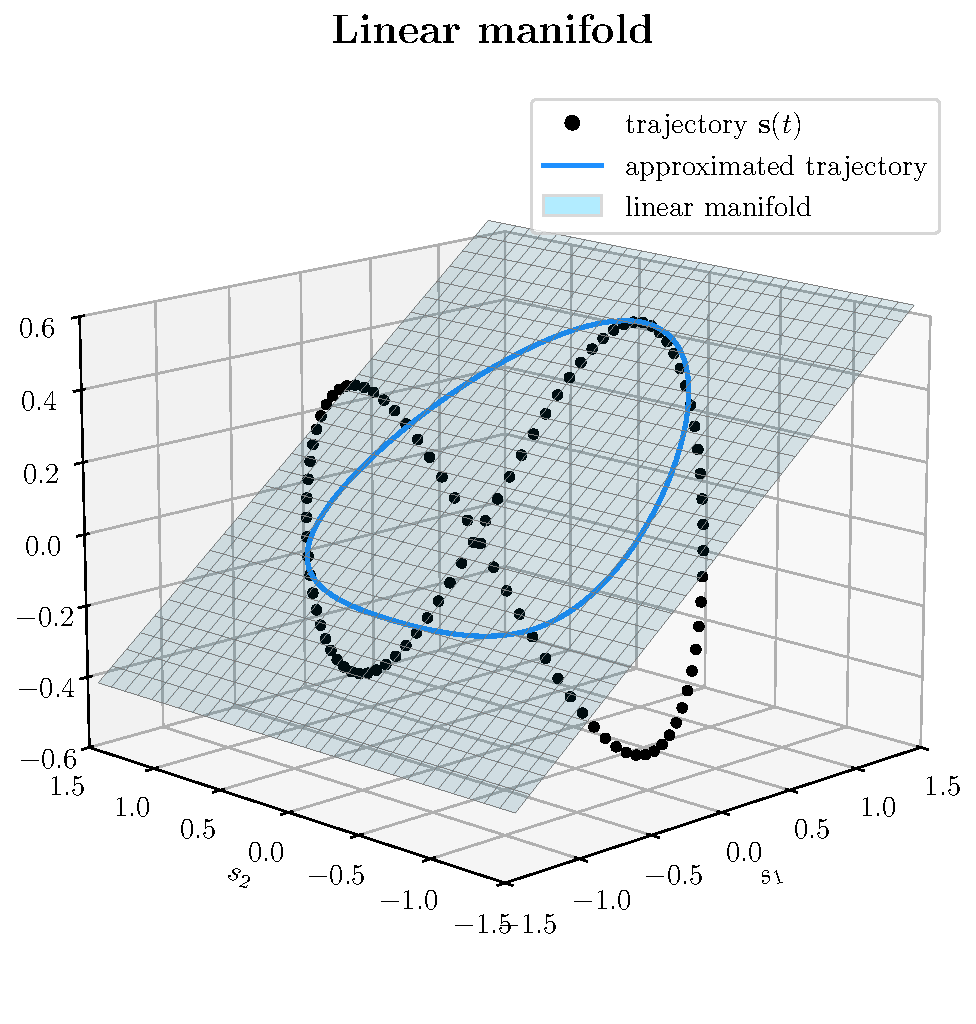
\includegraphics[width=0.45\textwidth]{Figures/linear_manifold.pdf}
  \caption{Global linear manifold (rank-2 plane) approximation of the 3D trajectory. The plane does not fully capture the redundant local curvature.}
  \label{fig:toy_linear_manifold}
\end{figure}

\vspace{0.5em}

\noindent
\textbf{Piecewise-linear manifold approximation.}  
To address this, the trajectory is partitioned into \(N_{\text{local}} = 4\) overlapping segments along the parameter \(t\).  
A local rank-2 POD basis is then constructed for each segment, creating a local linear manifold that best fits that region.  
By blending the local reconstructions in the overlap regions, the piecewise-linear manifold effectively captures the redundant structure and reconstructs the full closed trajectory with negligible error. Figures~\ref{fig:toy_local_manifold1}--\ref{fig:toy_local_manifold4} show each local manifold and its local reconstruction.

\begin{figure}[ht!]
  \centering
  \begin{subfigure}[b]{0.24\textwidth}
    \centering
    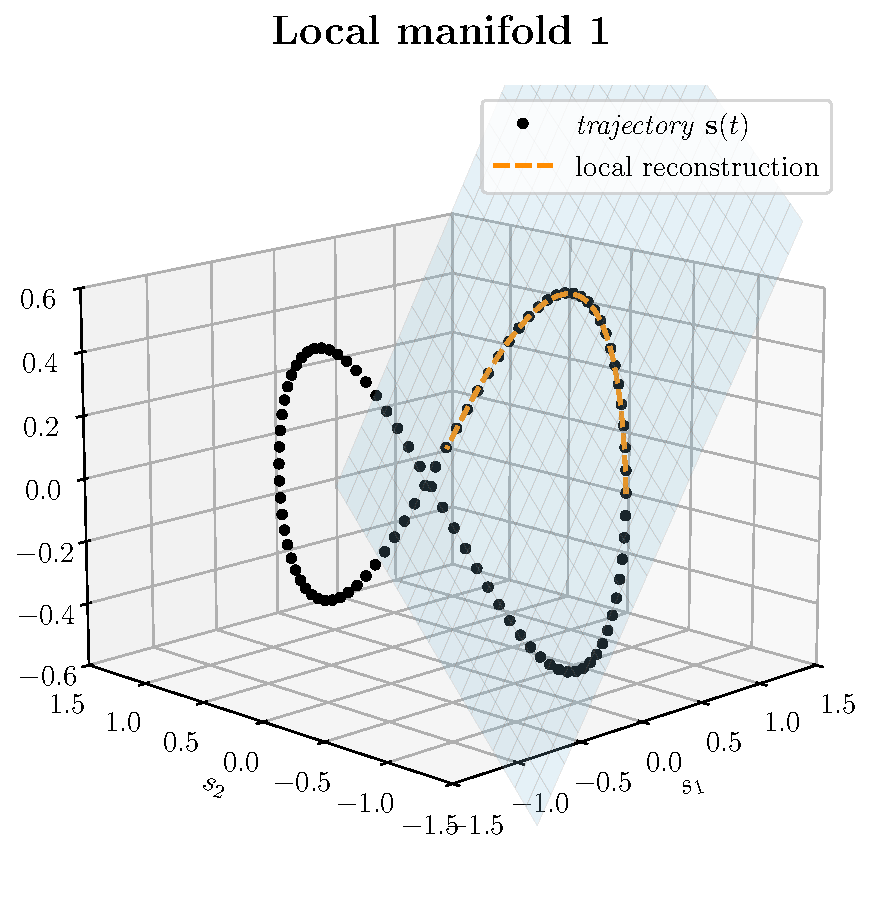
\includegraphics[width=\textwidth]{Figures/local_manifold_1.pdf}
    \caption{Local 1}
    \label{fig:toy_local_manifold1}
  \end{subfigure}
  \hfill
  \begin{subfigure}[b]{0.24\textwidth}
    \centering
    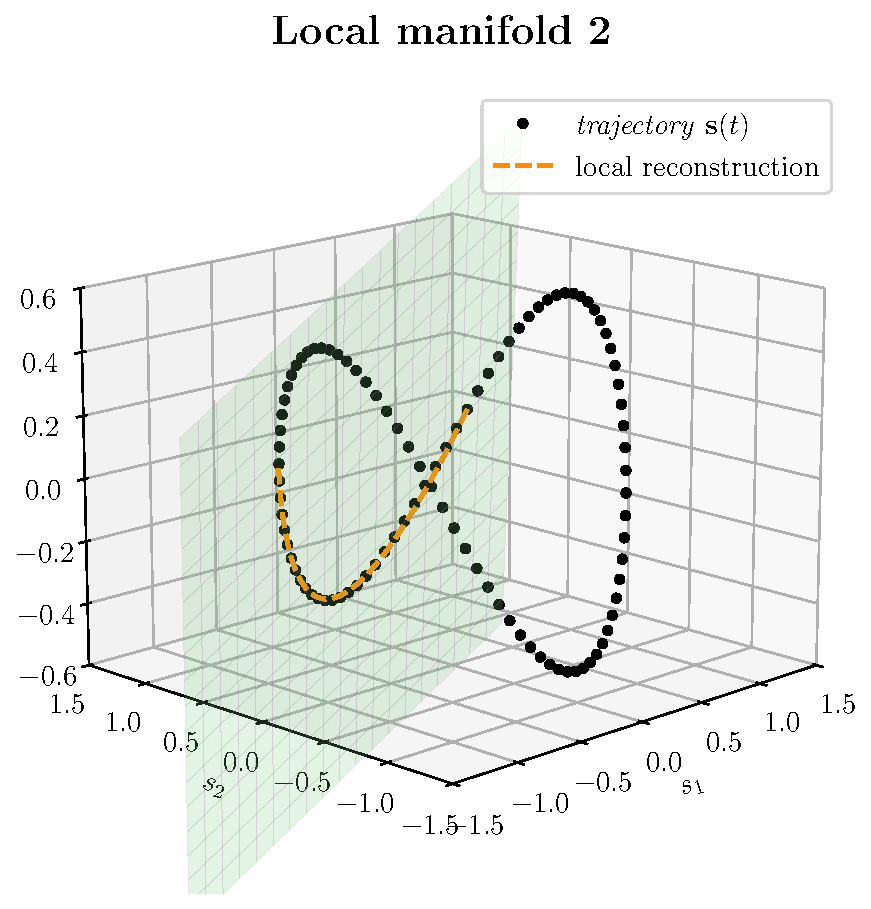
\includegraphics[width=\textwidth]{Figures/local_manifold_2.pdf}
    \caption{Local 2}
    \label{fig:toy_local_manifold2}
  \end{subfigure}
  \hfill
  \begin{subfigure}[b]{0.24\textwidth}
    \centering
    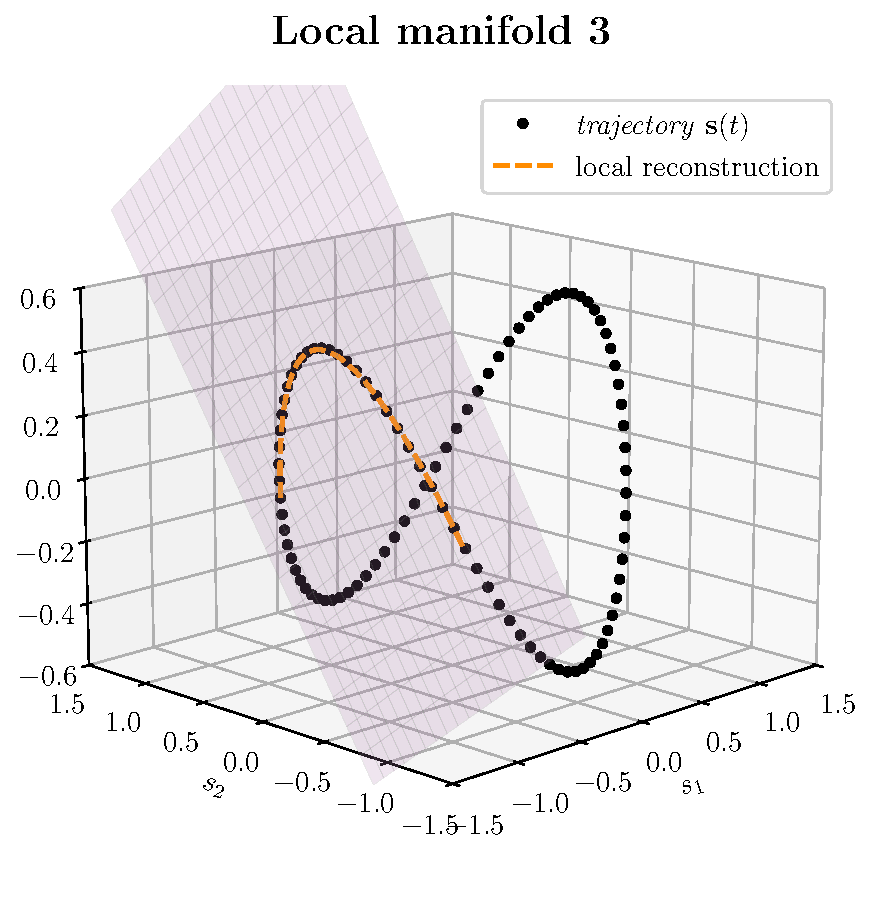
\includegraphics[width=\textwidth]{Figures/local_manifold_3.pdf}
    \caption{Local 3}
    \label{fig:toy_local_manifold3}
  \end{subfigure}
  \hfill
  \begin{subfigure}[b]{0.24\textwidth}
    \centering
    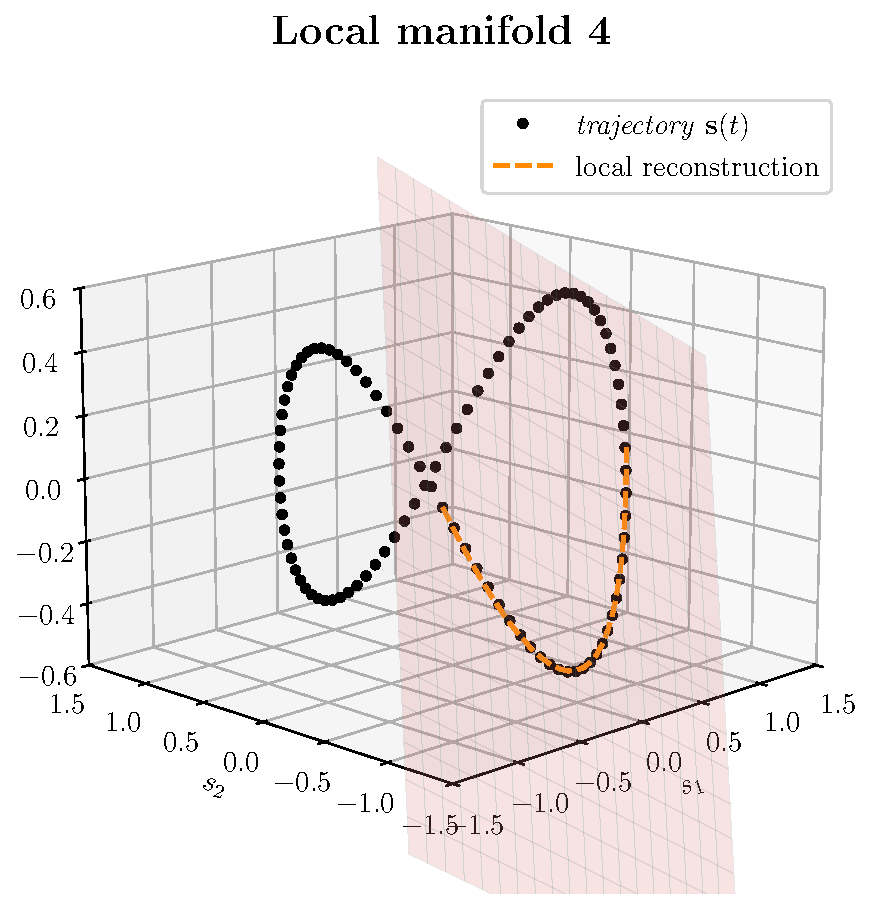
\includegraphics[width=\textwidth]{Figures/local_manifold_4.pdf}
    \caption{Local 4}
    \label{fig:toy_local_manifold4}
  \end{subfigure}

  \caption{Piecewise-local manifold approximations for segments 1--4 (horizontal layout).}
  \label{fig:toy_local_manifolds_all_horizontal}
\end{figure}

Finally, Figure~\ref{fig:toy_piecewise_combined} shows the combined piecewise-linear manifold and the blended approximation, which closely matches the original closed trajectory.  
This simple example highlights how local manifold approaches can overcome the approximation barrier imposed by the Kolmogorov \(n\)-width for problems with local nonlinear features.

\begin{figure}[ht!]
  \centering
  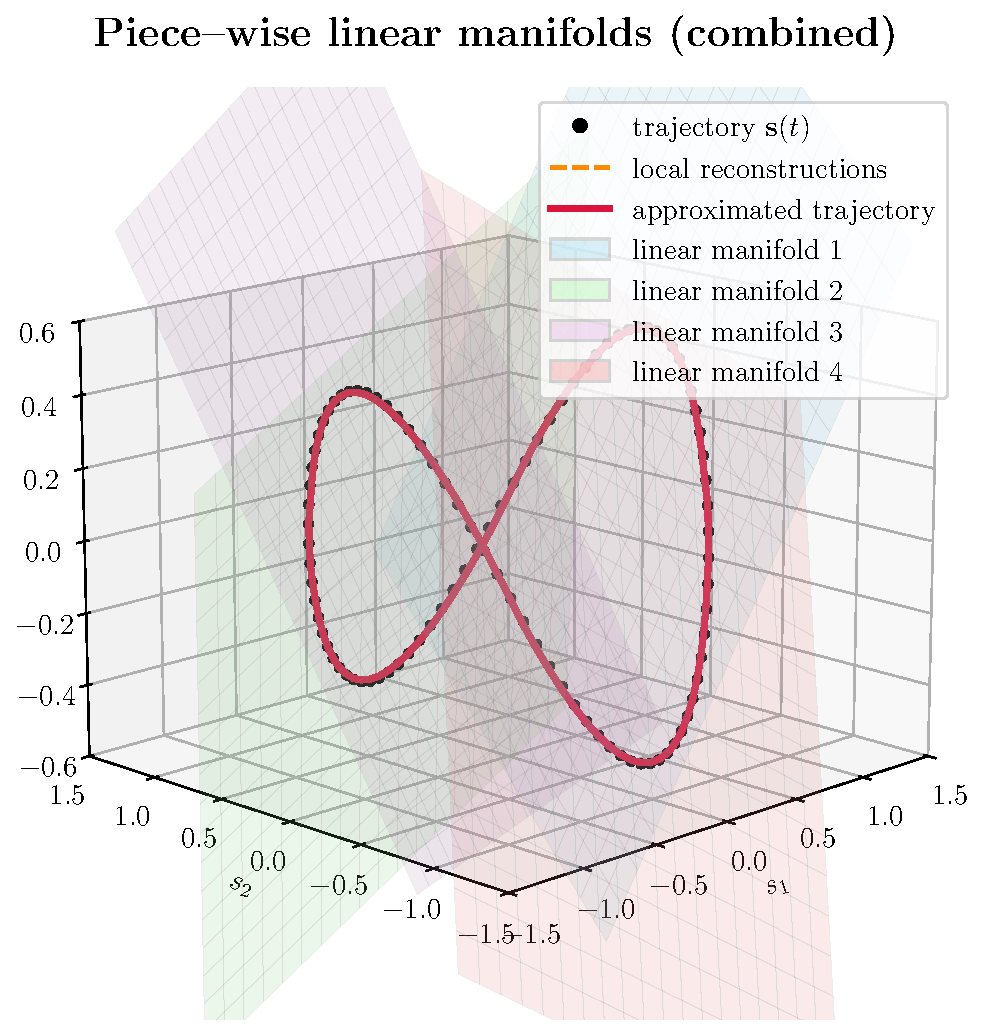
\includegraphics[width=0.45\textwidth]{Figures/piecewise_linear_combined.pdf}
  \caption{Combined piecewise-linear manifold approximation using four local POD bases with overlap. The blended local subspaces collectively recover the full 3D trajectory with minimal error.}
  \label{fig:toy_piecewise_combined}
\end{figure}

\subsection{Local POD PROM for the model problem}

Having established how piecewise-linear manifold approximations can overcome the limitations of a single global linear subspace, we now test this concept on the model problem introduced earlier.  
The inviscid one-dimensional Burgers’ equation, with its sharp gradients and convection-dominated character, provides an ideal setting to evaluate how local bases can reduce the approximation barrier imposed by the Kolmogorov~$n$-width.

In the offline stage, the full-order snapshot matrix is first projected onto a global POD basis, yielding reduced coordinates $\mathbf{q}_{g}$.  
A k-means clustering algorithm partitions these reduced coordinates into distinct clusters, with overlapping assignments to ensure smooth transitions across local bases.  
A local SVD is then performed for each cluster, retaining modes up to a common squared tolerance~$\epsilon^2$.

Figure~\ref{fig:average_modes_clusters} shows how the average number of modes per cluster changes as the number of clusters increases.  
A configuration with 20 clusters and an average of approximately 17.5 modes per cluster was selected, striking a balance between local adaptability and practical offline cost.

\begin{figure}[htbp]
    \centering
    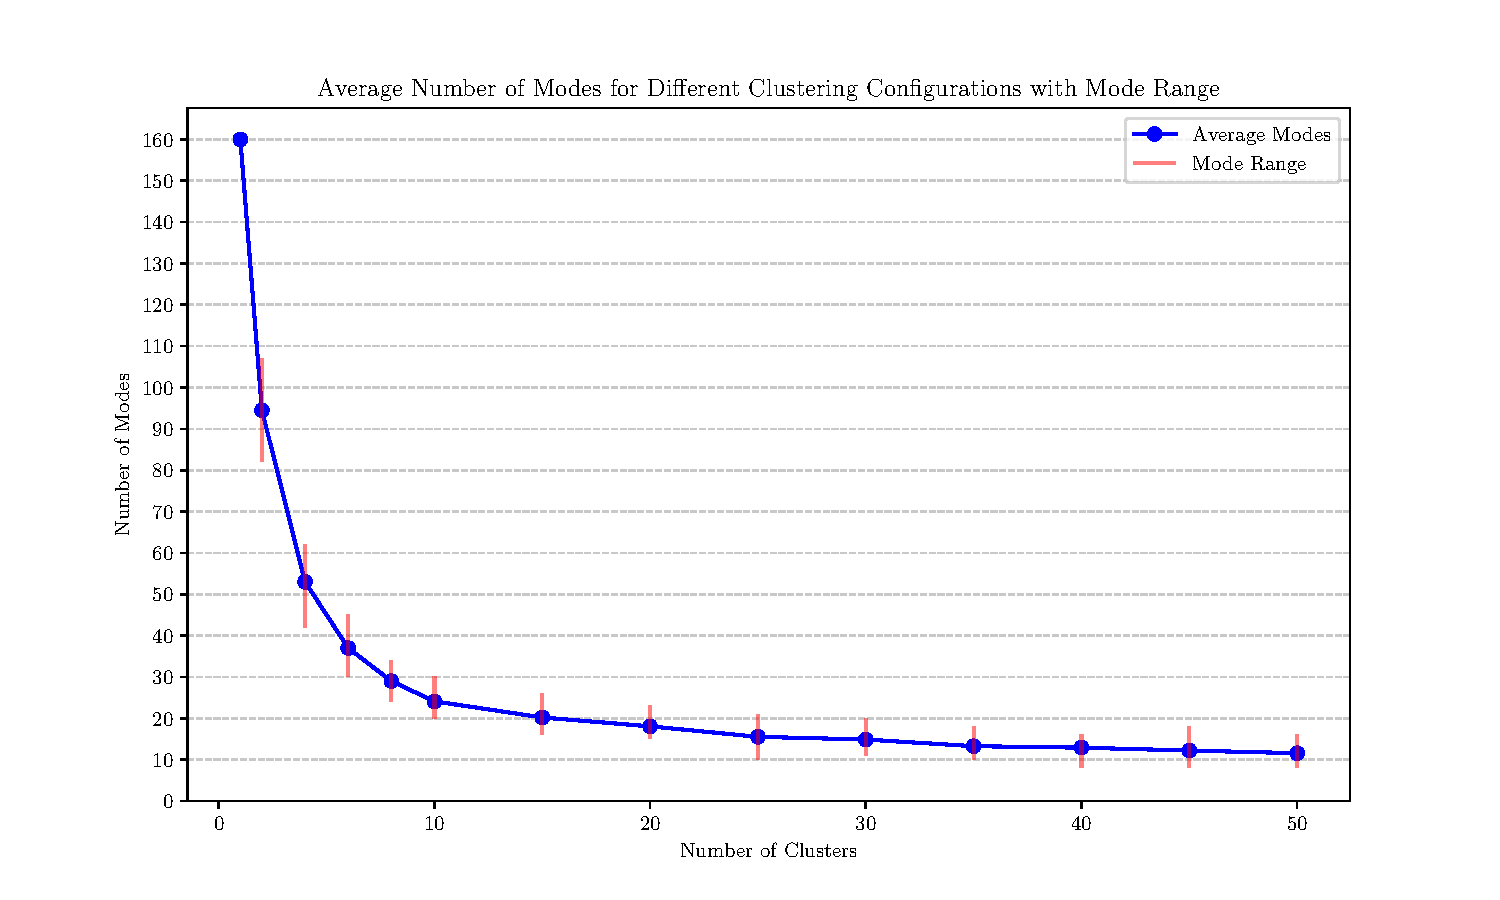
\includegraphics[width=0.7\textwidth]{Figures/average_modes_per_clustering_with_range.pdf}
    \caption{Average number of modes per cluster for different clustering configurations. Vertical bars indicate the range within each setup.}
    \label{fig:average_modes_clusters}
\end{figure}

For illustration, Figure~\ref{fig:fom_vs_local_global_pod} compares the full-order solution with its global and local PROM approximations for a representative parameter point~$\boldsymbol{\mu}_3 = [5.190,\,0.0260]$.  
The local approach visibly improves the resolution of steep wave fronts, demonstrating how local subspace partitioning adapts more effectively to convection-dominated features without requiring a significantly larger reduced dimension.

\begin{figure}[ht!]
    \centering
    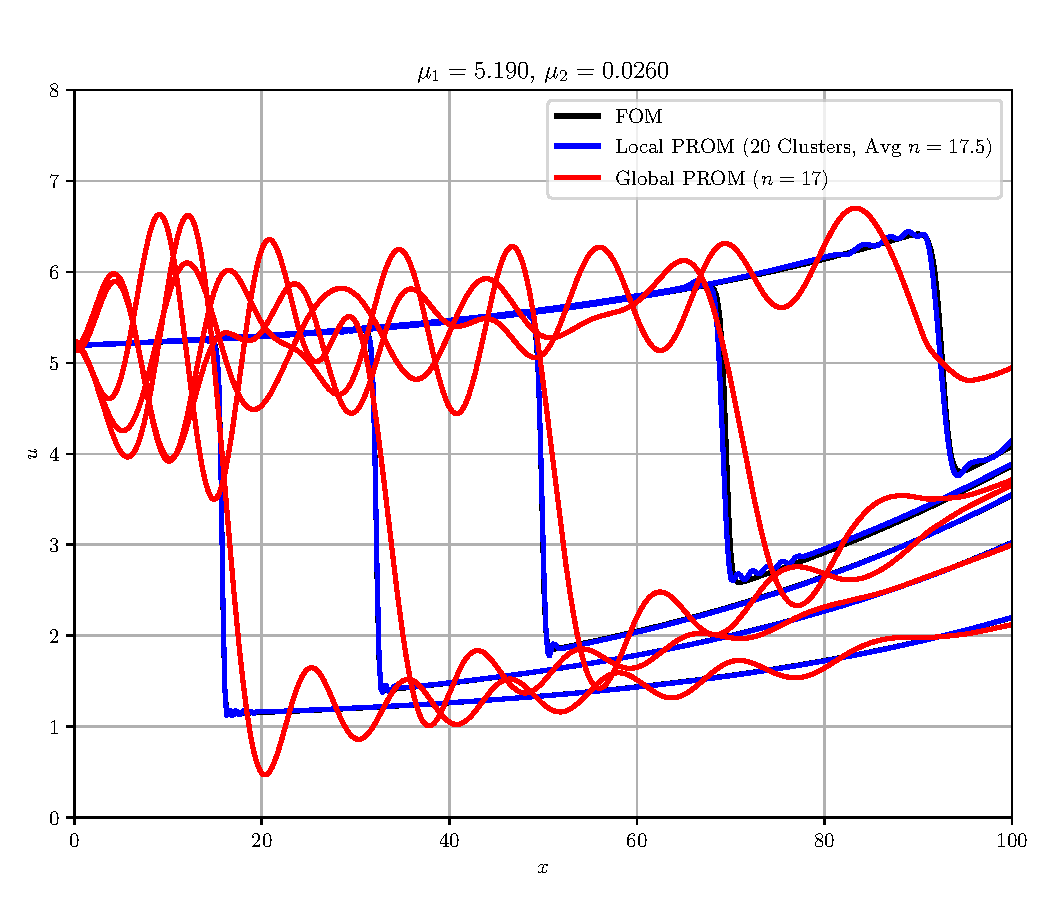
\includegraphics[width=0.7\textwidth]{Figures/fom_local_vs_global_pod_comparison_17_modes.pdf}
    \caption{Comparison of the FOM solution with the global PROM (17 modes) and the local PROM (20 clusters, average 17.5 modes) for $\mu_1 = 5.190$ and $\mu_2 = 0.0260$.}
    \label{fig:fom_vs_local_global_pod}
\end{figure}

Table~\ref{tab:local_global_pod_error_summary} summarizes the maximum relative $L_2$ error computed across three representative test configurations.  
The local PROM consistently achieves a substantial reduction in the worst-case error compared to the global basis while maintaining the same approximate basis size.

\begin{table}[htbp]
    \centering
    \begin{tabular}{c c c}
        \toprule
        Computational model & $n$ & $\mathbb{RE}^{\textbf{max}}_{2, \mathbf{u}}$ (\%) \\
        \midrule
        Global PROM & 17 & 13.52 \\
        Local PROM (20 Clusters) & 17.5 & 1.63 \\
        \bottomrule
    \end{tabular}
    \caption{Relative $L_2$ error across three test configurations for the global and local PROMs (LSPG). Maximum values across the points $\boldsymbol{\mu}_1 = [4.75,\, 0.0200]$, $\boldsymbol{\mu}_2 = [4.56,\, 0.0190]$, and $\boldsymbol{\mu}_3 = [5.19,\, 0.0260]$ are shown.}
    \label{tab:local_global_pod_error_summary}
\end{table}

\begin{table}[htbp]
\centering
\begin{tabular}{l c c}
    \toprule
        Computational model & $n$ & $\mathbb{RE}^{\textbf{max}}_{2, \mathbf{u}}$ (\%) \\
        \midrule
        Global PROM & 17 & 13.52 \\
        Local PROM (20 Clusters) & 17.5 & 1.63 \\
        \bottomrule
\end{tabular}

\medskip
{\small
Relative $L_2$ errors for the three test cases comparing the global and local PROMs.
}
\end{table}


These results confirm that piecewise-linear local PROMs offer a compelling and practical alternative to a single global subspace, especially for convection-dominated and transport problems where the Kolmogorov $n$-width is inherently large. While clustering, overlap, and online basis selection introduce additional offline complexity, these aspects remain manageable and justified by the improved accuracy and stability that local Petrov--Galerkin projections provide. From the hyper-reduction perspective, the local framework integrates well with ECSW-type methods~\cite{grimberg2021mesh}, which rigorously construct element-wise sampling sets through a convex formulation with minimal tuning parameters. This approach supports either a single reduced mesh shared by all local bases, or multiple reduced meshes adapted to each subspace, providing flexibility in balancing accuracy and online cost.

\textbf{As an additional contribution, I co-authored a related work~\cite{bravo2024subspace}} that proposes a novel subspace-adaptive weights cubature method, building on the ECM framework. This extension enables multiple local bases to share a common reduced mesh with tailored weights for each subspace. The resulting approach provides a robust third option for local hyper-reduction and demonstrates scalable performance for highly nonlinear problems, further reinforcing the practicality of local PROMs in large-scale applications.

% \section{Autoencoder-based nonlinear manifolds}

\section{Quadratic manifolds}

Quadratic approximation manifolds have emerged as a promising strategy for overcoming the limitations imposed by the Kolmogorov $n$-width barrier by extending the traditional affine approximation with explicit quadratic terms in the reduced coordinates. These models introduce controlled curvature into the solution representation, enabling more compact and accurate reduced-order models. Early developments in this area include simulation-free formulations for nonlinear structural dynamics problems~\cite{jain2017quadratic}, as well as fully data-driven versions tailored to large-scale CFD applications with transport phenomena~\cite{barnett2022quadratic}. 

Notably, the integration of quadratic approximation manifolds with robust projection and hyper-reduction frameworks, such as the LSPG projection~\cite{carlberg2011efficient} and energy-conserving sampling and weighting (ECSW)~\cite{grimberg2021mesh}, has demonstrated substantial speed-ups and high accuracy for challenging benchmarks like the Ahmed body turbulent wake~\cite{barnett2022quadratic} and hypersonic flow predictions~\cite{chmiel2025unified}. These results illustrate the potential of quadratic manifolds to deliver orders-of-magnitude performance improvements compared to conventional affine PROMs while remaining interpretable, simulation-driven, and relatively data-efficient.

In the following sections, we formalize the general quadratic manifold decoder, derive its associated minimum-residual projection, and present a representative toy example that highlights its ability to capture nonlinear solution features that lie beyond the reach of linear subspaces. Finally, the approach is evaluated for the one-dimensional inviscid Burgers’ equation, providing a consistent comparison to the linear and piecewise-linear strategies discussed earlier.

\subsection{Quadratic manifold formulation}
\label{sec:quad_manifold_formulation}

The quadratic manifold extends the traditional linear subspace approximation by enriching the solution representation with second-order terms in the reduced coordinates. Specifically, the quadratic approximation (decoder) is defined as:
%
\begin{equation}
\tilde{\mathbf{u}}(t,\boldsymbol{\mu}) =
\mathbf{u}_{\text{ref}} +
\boldsymbol{\Phi}\,\mathbf{q}(t,\boldsymbol{\mu}) +
\mathbf{H}\,\bigl(\mathbf{q}(t,\boldsymbol{\mu})\otimes\mathbf{q}(t,\boldsymbol{\mu})\bigr),
\quad
\boldsymbol{\Phi}\in\mathbb{R}^{N\times n},\;
\mathbf{H}\in\mathbb{R}^{N\times n^{2}},
\label{eq:quad_decoder_full}
\end{equation}
%
where $\mathbf{u}_{\text{ref}}\in\mathbb{R}^{N}$ is a chosen reference state (e.g., mean flow or steady-state solution), 
$\boldsymbol{\Phi}$ is the linear POD basis, and $\mathbf{H}$ is a second-order tensor reshaped as a matrix. For notational simplicity, the following derivations will assume $\mathbf{u}_{\text{ref}}=0$ and will omit explicit dependence on $t$ and $\boldsymbol{\mu}$, unless required for clarity.
The term $\mathbf{q}\otimes\mathbf{q}\in\mathbb{R}^{n^{2}}$ denotes the full Kronecker product, explicitly containing all quadratic monomials:
%
\[
\mathbf{q}\otimes\mathbf{q}=
\begin{bmatrix}
q_1^2,\,q_1 q_2,\,\dots,\,q_1 q_n,\,
q_2 q_1,\,q_2^2,\,\dots,\,q_n^2
\end{bmatrix}^T.
\]

However, this representation introduces redundancy since cross-terms such as \(q_i q_j\) and \(q_j q_i\) appear twice. To remove this redundancy, we employ the symmetric quadratic monomial vector:
%
\begin{equation}
\mathbf{Q}_s(\mathbf{q}) =
\begin{bmatrix}
q_1^{2},\, q_1 q_2,\, q_1 q_3,\, \dots,\, q_2^2,\,\dots,\,q_n^{2}
\end{bmatrix}^{T}\in\mathbb{R}^{k}, \quad k=\frac{n(n+1)}{2}.
\label{eq:symmetric_monomials}
\end{equation}

With this symmetric representation, the quadratic decoder becomes:
%
\begin{equation}
D_u(\mathbf{q}) =
\boldsymbol{\Phi}\mathbf{q} +
\mathbf{H}_s\,\mathbf{Q}_s(\mathbf{q}),
\quad \mathbf{H}_s\in\mathbb{R}^{N\times k}.
\label{eq:quad_decoder_sym}
\end{equation}

\paragraph{Practical selection of the latent dimension.}
Given a POD energy tolerance $\epsilon$ and a padding factor $\zeta$, 
we first compute the smallest integer $n_{\text{tra}}$ such that the leading
$n_{\text{tra}}$ singular values capture at least $(1-\epsilon)$ of the
snapshot energy.  
Since a quadratic manifold with $n$ primary coordinates contains
$k=\tfrac{n(n+1)}{2}$ distinct quadratic monomials, we choose the minimal $n$
satisfying $k \ge n_{\text{tra}}$ and then inflate it by the factor
$(1+\zeta)$ to provide headroom for additional variance.  
Finally, an upper bound 
$
n \le n_{\max}=\frac{\sqrt{1+8N_s}-1}{2}
$
is enforced so that the symmetric-Kronecker matrix has at least as many rows
as snapshots, keeping the ridge-regression system well posed.


\textbf{Offline construction of the quadratic manifold} The quadratic manifold is constructed from the available snapshot set by determining the linear basis \(\boldsymbol{\Phi}\) and the quadratic coefficient tensor \(\mathbf{H}_s\). For each of the \(N_s\) snapshots, we first define the linear reconstruction errors:
%
\[
\mathbf{e}_\ell =
\mathbf{u}_\ell - \boldsymbol{\Phi}\mathbf{q}_\ell,
\quad \ell=1,\dots,N_s,
\]
%
which are collected into the error matrix:
%
\[
\mathbf{E} =
\begin{bmatrix}
\mathbf{e}_1 & \dots & \mathbf{e}_m
\end{bmatrix}\in\mathbb{R}^{N\times N_s}.
\]

To identify the quadratic terms, we construct a symmetric quadratic regression matrix:
%
\[
\mathbf{Z} =
\begin{bmatrix}
\mathbf{Q}_s(\mathbf{q}_1) & \dots & \mathbf{Q}_s(\mathbf{q}_m)
\end{bmatrix}\in\mathbb{R}^{k\times N_s},
\]
%
where each column \(\mathbf{Q}_s(\mathbf{q}_\ell)\) contains the unique quadratic monomials defined in \eqref{eq:symmetric_monomials} evaluated at \(\mathbf{q}_\ell\).

The quadratic coefficient tensor \(\mathbf{H}_s\) is determined by solving the regularized least-squares (ridge regression) problem:
%
\[
\min_{\mathbf{H}_s}\|\mathbf{E}-\mathbf{H}_s\mathbf{Z}\|_F^2+\alpha^2\|\mathbf{H}_s\|_F^2,
\]
%
where \(\alpha>0\) is the Tikhonov regularization parameter. This problem admits a closed-form solution obtained via the thin SVD \(\mathbf{Z}= \mathbf{U}_z\boldsymbol{\Sigma}_z\mathbf{V}_z^T\):
%
\begin{equation}
\mathbf{H}_s=
(\mathbf{U}_z\operatorname{diag}(f))
\left(\mathbf{V}_z^T\mathbf{E}^T/\boldsymbol{\Sigma}_z\right)^T,
\quad
f_\ell=\frac{\sigma_\ell^2}{\sigma_\ell^2+\alpha^2},\, \ell=1,\dots,r.
\label{eq:H_closedform}
\end{equation}

Here, the division by \(\boldsymbol{\Sigma}_z\) denotes element-wise division by each singular value.

\textbf{Derivative of the quadratic decoder} The derivative of the quadratic decoder \eqref{eq:quad_decoder_full} with respect to the reduced coordinates \(\mathbf{q}\) in the full Kronecker form is initially expressed as:
%
\begin{equation}
\frac{\partial\tilde{\mathbf{u}}}{\partial\mathbf{q}}(\mathbf{q}) =
\boldsymbol{\Phi} +
\mathbf{H}\left[\mathbf{q}\otimes\mathbf{I}+\mathbf{I}\otimes\mathbf{q}\right],
\label{eq:quad_derivative_full}
\end{equation}
%
with \(\mathbf{I}\) the \(n\times n\) identity.

However, employing the symmetric quadratic monomial vector \(\mathbf{Q}_s(\mathbf{q})\), the derivative simplifies to a compact form directly suitable for efficient computation:
%
\begin{equation}
\frac{\partial D_u}{\partial\mathbf{q}} =
\boldsymbol{\Phi} +
\mathbf{H}_s\,\frac{\partial\mathbf{Q}_s}{\partial\mathbf{q}},
\quad
\frac{\partial\mathbf{Q}_s}{\partial\mathbf{q}}\in\mathbb{R}^{k\times n}.
\label{eq:quad_derivative_sym}
\end{equation}

Each row of the matrix \(\partial\mathbf{Q}_s/\partial\mathbf{q}\) is derived analytically as follows:

\begin{itemize}
    \item Diagonal terms: \(\displaystyle\frac{\partial(q_i^2)}{\partial q_i}=2q_i.\)
    \item Off-diagonal terms (\(j>i\)): 
    \(\displaystyle\frac{\partial(q_i q_j)}{\partial q_i}=q_j,\quad \frac{\partial(q_i q_j)}{\partial q_j}=q_i.\)
\end{itemize}

\paragraph{LSPG minimum-residual projection on quadratic manifolds}

The quadratic manifold PROM (QPROM) adopts the same minimum-residual projection framework introduced in Section~\ref{subsec:minres-manifold-rom}. At each online time step, the reduced coordinates are updated via a Gauss--Newton iteration that solves:
\begin{equation}
\Bigl(\frac{\partial D_u}{\partial\mathbf{q}}\Bigr)^{(k)T} 
\mathbf{J}^{(k)T} \mathbf{J}^{(k)}
\Bigl(\frac{\partial D_u}{\partial\mathbf{q}}\Bigr)^{(k)}
\,\delta\mathbf{q}^{(k)}
= 
-\Bigl(\frac{\partial D_u}{\partial\mathbf{q}}\Bigr)^{(k)T}
\mathbf{J}^{(k)T}\mathbf{R}^{(k)},
\label{eq:lspg_quad_proj}
\end{equation}
where the decoder derivative $\partial D_u/\partial \mathbf{q}$ follows its definition in Eq.~\eqref{eq:quad_derivative_sym}. This ensures a consistent and robust minimum-residual projection for quadratic manifold approximations.


\subsection{Illustrative toy example: quadratic manifold on a redundant 3D trajectory}

We revisit the illustrative example of Section~\ref{sec:piecewise_linear}, employing a quadratic manifold approximation instead of a piecewise-linear one. The trajectory \(\mathbf{s}(t)\) remains the same, embedding a closed curve in three-dimensional space with a nonlinear dependency that prevents accurate representation by a single linear subspace. First, a global rank-2 POD basis is obtained from the snapshot data as before. Rather than partitioning the manifold, we enrich this global linear representation by introducing quadratic terms, resulting in a single curved manifold (a paraboloid). Figure~\ref{fig:toy_quadratic_manifold} shows the resulting quadratic manifold, clearly demonstrating its improved capacity to represent the original trajectory without the need for multiple local bases.

\begin{figure}[ht!]
  \centering
  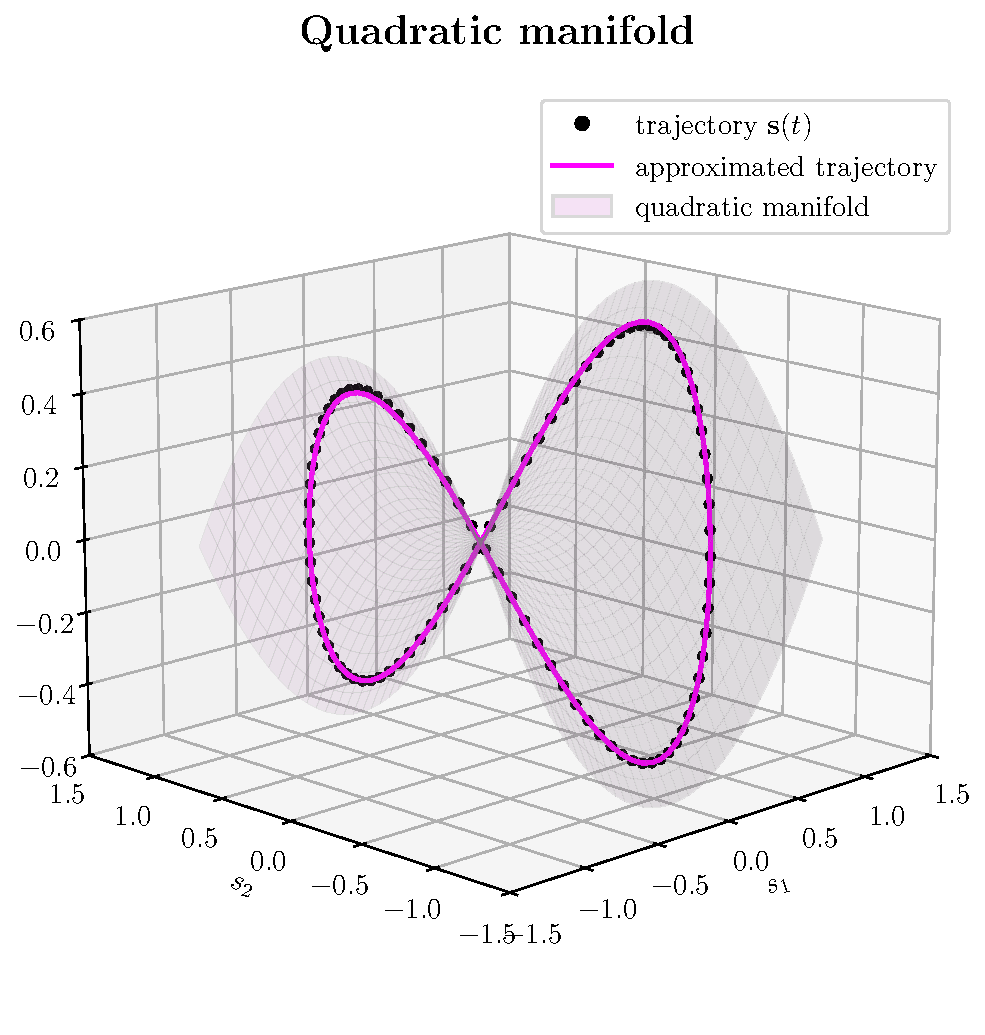
\includegraphics[width=0.6\textwidth]{Figures/quadratic_manifold.pdf}
  \caption{Quadratic manifold approximation of the 3D trajectory. By enriching the global linear subspace with quadratic terms, the manifold accurately captures the local curvature inherent in the trajectory.}
  \label{fig:toy_quadratic_manifold}
\end{figure}

Compared to the linear manifold approximation, the quadratic manifold achieves a significantly reduced approximation error due to its intrinsic ability to represent nonlinear solution structures. This simple yet illustrative example highlights the power of quadratic manifold approximations in overcoming the limitations imposed by the Kolmogorov \(n\)-width barrier, without the complexity associated with piecewise or local constructions.


\subsection{Quadratic manifold PROM for the model problem}

Having demonstrated the potential of quadratic manifold approximations to represent nonlinear solution features efficiently, we now evaluate this approach on the one-dimensional inviscid Burgers’ equation introduced previously as the model problem. The convection-dominated character and sharp gradients of this test case provide a stringent setting to assess the effectiveness of the quadratic manifold in addressing the limitations associated with global linear subspace approximations.

The offline construction begins by applying POD to the snapshot dataset, yielding a global linear subspace \(\boldsymbol{\Phi}\). The quadratic manifold tensor \(\mathbf{H}_s\) is then identified through regularized regression, following the procedure described in Section~\ref{sec:quad_manifold_formulation}. Using a POD energy tolerance of $\epsilon = 10^{-6}$ and a 10\% padding factor ($\zeta = 0.1$), the automatic dimension-selection procedure described in Section~\ref{sec:quad_manifold_formulation} yields $n = 21$ retained coordinates for the QPROM. This value balances reconstruction accuracy with computational cost while ensuring the quadratic regression system is well posed.


Figure~\ref{fig:fom_vs_quadratic_rom} compares the FOM solution with both the QPROM and a global linear POD PROM for the representative test case \(\boldsymbol{\mu} = [4.750,\,0.0200]\). Clearly, the quadratic manifold approximation significantly improves the resolution of the nonlinear features of the solution, capturing steep gradients and sharp wave fronts more accurately than the linear PROM.

\begin{figure}[htbp]
    \centering
    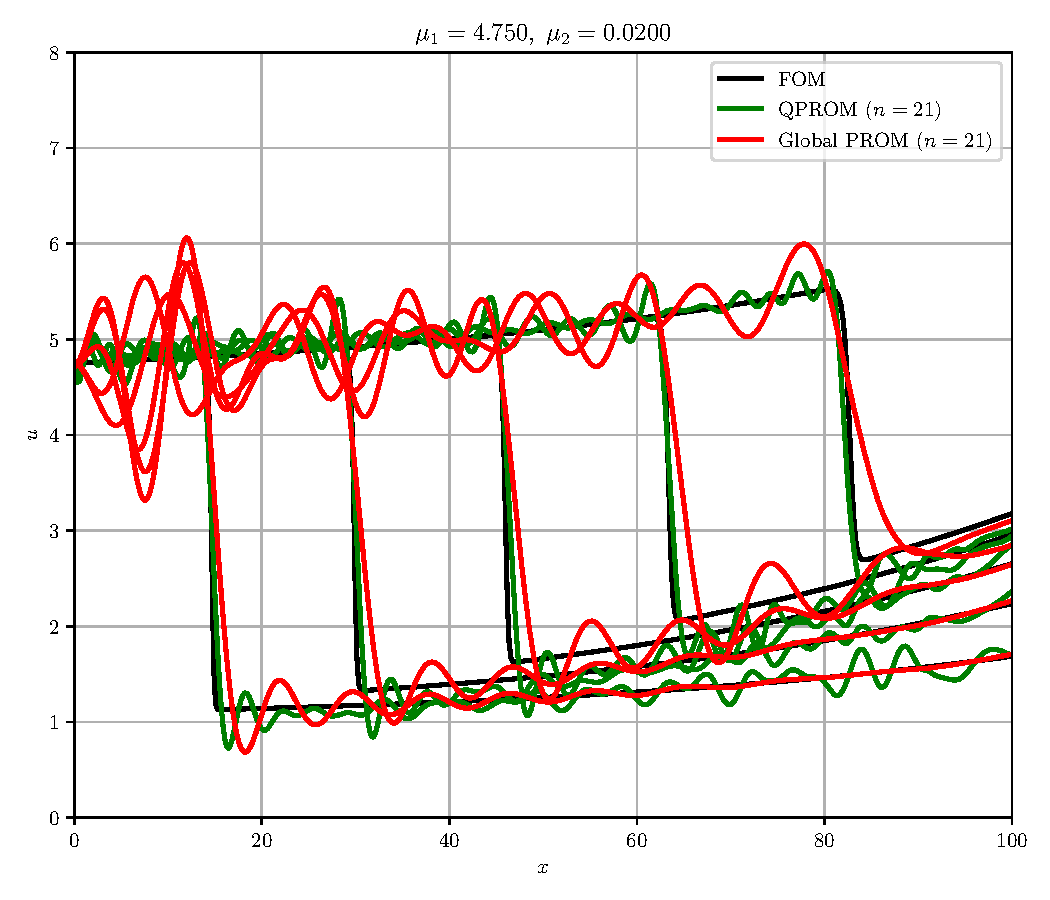
\includegraphics[width=0.7\textwidth]{Figures/fom_vs_qprom_mu1_4.750_mu2_0.0200.pdf}
    \caption{Comparison of the FOM solution with the QPROM (21 modes) and the global linear PROM (21 modes) for the parameter set \(\mu_1 = 4.750\), \(\mu_2 = 0.0200\).}
    \label{fig:fom_vs_quadratic_rom}
\end{figure}

Table~\ref{tab:quad_vs_global_pod_error_summary} summarizes the maximum relative \(L_2\) error computed across three representative test configurations. The quadratic manifold consistently achieves significant error reduction compared to the global linear POD PROM, clearly demonstrating its capability to overcome the approximation barrier posed by the Kolmogorov \(n\)-width with modest computational effort.

\begin{table}[htbp]
    \centering
    \begin{tabular}{c c c}
        \toprule
        Computational Model & $n$ & $\mathbb{RE}^{\textbf{max}}_{2, \mathbf{u}}$ (\%) \\
        \midrule
        Global PROM & 21 & 9.74 \\
        QPROM & 21 & 4.67 \\
        \bottomrule
    \end{tabular}
    \caption{Maximum relative \(L_2\) error computed across the three test parameter sets \(\boldsymbol{\mu}_1 = [4.750,\, 0.0200]\), \(\boldsymbol{\mu}_2 = [4.560,\, 0.0190]\), and \(\boldsymbol{\mu}_3 = [5.190,\, 0.0260]\).}
    \label{tab:quad_vs_global_pod_error_summary}
\end{table}


These results highlight the QPROM as a compelling and practical alternative to global linear subspace approaches. By explicitly introducing controlled nonlinear curvature through quadratic terms, this method substantially reduces approximation errors over purely linear representations, circumventing the dimensional limitations associated with linear subspaces, without introducing the complexity of clustering or local basis selection inherent to local POD methods. Furthermore, the quadratic manifold integrates naturally with hyper-reduction techniques such as ECSW or ECM, facilitating scalable and efficient implementations for large-scale industrial applications~\cite{barnett2022quadratic,chmiel2025unified}.

However, the quadratic manifold approach still has limitations. While its effectiveness is notable for problems exhibiting mild to moderate nonlinearities, highly complex phenomena, such as strong discontinuities, shock-shock interactions, or intricate parametric dependencies, may require even richer representations. In such cases, a single quadratic manifold may be insufficient, and extensions like piecewise quadratic approximations or fully nonlinear latent-space models based on machine learning regressors may be needed. This motivates the exploration of nonlinear latent-space closure modeling approaches in the next section, which aim to combine the robustness of projection-based formulations with the expressivity of modern machine learning architectures. In particular, recent results for the hypersonic double-cone problem~\cite{chmiel2025unified}, featuring shock-shock interactions and multiple nonlinear flow phenomena, demonstrate that, although the quadratic manifold reduces the number of retained modes from 16 to 12 compared to a standard PROM, it is ultimately outperformed by a PROM-ANN~\cite{barnett2023neural, chmiel2025unified} model using only 2 latent variables, achieving superior speed-ups and accuracy.


\section{Nonlinear manifold construction via latent-space closure modeling with neural networks}
\label{sec:latent_nn}

While quadratic manifold approaches provide a structured yet limited means of modeling closure errors by explicitly defining a quadratic dependence on generalized coordinates, a more general strategy is to represent the closure error using flexible, nonlinear functions learned directly from data. In this context, neural-network-based latent-space closure modeling emerges naturally as a powerful extension of previously discussed manifold formulations, particularly effective for problems exhibiting complex nonlinear behaviors, strong convection, or shocks.

Several neural-network-based methods have recently been proposed for constructing nonlinear approximation manifolds. Among them, convolutional autoencoder architectures \cite{lee2020model, romor2023non} represent an influential direction, utilizing deep convolutional neural networks to embed high-dimensional solutions into low-dimensional nonlinear manifolds. Lee and Carlberg \cite{lee2020model} successfully applied deep convolutional autoencoders to dynamical systems, while Romor et al. \cite{romor2023non} combined convolutional autoencoders with a reduced over-collocation method, achieving notable results in fluid dynamics. However, these convolution-based approaches inherently scale poorly with increasing problem dimensionality, restricting their applicability in practice primarily to problems of moderate size, far below the scales encountered in typical industrial models with millions of degrees of freedom.

An alternative nonintrusive strategy that avoids this scalability bottleneck is the POD-DL-ROM framework~\cite{FRESCA2022114181}, which decouples spatial complexity from network training via a deep feedforward network acting on POD-reduced coordinates. While this model has shown promising results in various parametric problems, its fully nonintrusive nature still limits the incorporation of governing physics or residual consistency into the learning process.

Addressing these scalability and physics-integration limitations, Barnett et al.~\cite{barnett2023neural} introduced a novel latent-space closure framework within the PMOR paradigm. Their approach, known as PROM-ANN, utilizes deep ANNs to model the closure errors explicitly within the low-dimensional latent space, directly circumventing the computational burden associated with high-dimensional network training. By training only within the reduced latent coordinates, thus decoupling the training complexity from the dimension of the original HDM, this methodology achieves significant computational advantages and improved scalability. Moreover, unlike nonintrusive models, PROM-ANN preserves the intrusive structure of projection-based ROMs, enabling future extensions that embed physical constraints into the training procedure.


This framework was successfully demonstrated for challenging convection-dominated problems characterized by slow-decaying Kolmogorov $n$-widths, such as unsteady parametric shock-driven flows and hypersonic flow regimes \cite{barnett2023neural, chmiel2025unified}. In particular, Barnett et al.~\cite{barnett2023neural} illustrated the PROM-ANN capability by constructing hyperreduced PROMs (HPROM-ANNs) achieving superior accuracy compared to traditional affine-based HPROMs. Specifically, they demonstrated nearly three orders of magnitude acceleration over the underlying HDM with approximately 97\% accuracy, utilizing dramatically smaller reduced dimensions. Moreover, Chmiel et al.~\cite{chmiel2025unified} successfully extended this method to hypersonic flows governed by the Navier–Stokes equations, highlighting its effectiveness even at extremely low-dimensional manifolds.

This thesis builds directly upon these developments, exploring deeper methodological improvements and alternative strategies aimed at further enhancing performance, robustness, and interpretability of latent-space closure models. The subsequent subsections provide detailed formulation and illustrative examples of ANN-based latent-space closure, setting the stage for the proposed methodological extensions presented in the following chapters.


\subsection{Latent closure model formulation: ANN-based nonlinear manifolds}
\label{subsec:latent_ann_formulation}

As previously discussed, the general manifold projection-based reduced order modeling approach seeks solutions on nonlinear manifolds parametrized by reduced coordinates~$\mathbf{q}(t,\boldsymbol{\mu})$. In the latent-space closure framework~\cite{barnett2023neural, cohen2023nonlinear}, the approximation manifold is constructed by partitioning a global reduced-order basis $\boldsymbol{\Phi}_{\text{tot}}$, obtained via POD and energy truncation, into two orthogonal subspaces:
\begin{equation}
\boldsymbol{\Phi}_{\text{tot}} = [\,\boldsymbol{\Phi},\, \overline{\boldsymbol{\Phi}}\,], 
\quad 
\boldsymbol{\Phi} \in \mathbb{R}^{N \times n}, 
\quad 
\overline{\boldsymbol{\Phi}} \in \mathbb{R}^{N \times \bar{n}},
\quad 
n \ll \bar{n} \ll N.
\label{eq:basis_partition_latent}
\end{equation}
The columns of $\boldsymbol{\Phi}$ define the retained modes explicitly resolved by the PROM, while the columns of $\overline{\boldsymbol{\Phi}}$ correspond to discarded modes, whose influence is modeled nonlinearly. The resulting nonlinear decoder takes the form:
\begin{equation}
\mathbf{u}(t,\boldsymbol{\mu}) \approx \tilde{\mathbf{u}}(t,\boldsymbol{\mu}) 
= D_u(\mathbf{q}(t,\boldsymbol{\mu})) 
= \mathbf{u}_{\text{ref}} + \boldsymbol{\Phi}\,\mathbf{q}(t,\boldsymbol{\mu}) 
+ \overline{\boldsymbol{\Phi}}\,\mathcal{N}(\mathbf{q}(t,\boldsymbol{\mu})),
\label{eq:decoder_latent}
\end{equation}
where $\mathbf{u}_{\text{ref}} \in \mathbb{R}^N$ is a chosen reference state and 
$\mathcal{N}:\mathbb{R}^n\rightarrow\mathbb{R}^{\bar{n}}$ is a nonlinear closure map, in this case, realized by an artificial neural network.

Unless otherwise stated, and for notational simplicity, the following derivations will assume $\mathbf{u}_{\text{ref}}=0$ and will omit explicit dependence on $(t,\boldsymbol{\mu})$.



\paragraph{Construction of the latent-space closure via ANN}
The nonlinear closure map $\mathcal{N}$ can be effectively represented using machine learning regression methods, particularly ANNs. Given the solution snapshots $\{\mathbf{u}_{s}\}_{s=1}^{N_s}$, the primary and secondary generalized coordinates for training are computed by projection onto the partitioned basis:
\begin{equation}
\mathbf{q}_{s} = \boldsymbol{\Phi}^T \mathbf{u}_{s},\quad
\bar{\mathbf{q}}_{s} = \overline{\boldsymbol{\Phi}}^T \mathbf{u}_{s}, 
\quad s = 1,\dots,N_s.
\label{eq:proj_coordinates_ann}
\end{equation}


The ANN approximation of the nonlinear latent map is then trained by minimizing a mean-squared-error loss:
\begin{equation}
\boldsymbol{\eta}^{*} = \arg\min_{\boldsymbol{\eta}} 
\frac{1}{N_{\text{train}}}
\sum_{s=1}^{N_{\text{train}}}
\left\|
\bar{\mathbf{q}}_{s}
-
\mathcal{N}(\mathbf{q}_{s};\,\boldsymbol{\eta})
\right\|_{2}^{2},
\label{eq:ann_training}
\end{equation}
where $\boldsymbol{\eta}$ denotes the ANN parameters. Note that the dimension of this regression problem scales with $n$ and $\bar{n}$, independently of the HDM dimension $N$, ensuring scalability to large-scale models.


\paragraph{LSPG minimum-residual projection on ANN-based nonlinear manifolds}

Given the nonlinear decoder in Eq.~\eqref{eq:decoder_latent}, the LSPG minimum-residual projection follows the general residual minimization framework introduced in Section~\ref{subsec:minres-manifold-rom}. For ANN-based latent-space closures, the Gauss--Newton iteration for the reduced coordinates at each discrete time step reads:
\begin{equation}
\Bigl(\frac{\partial D_u}{\partial \mathbf{q}}\Bigr)^{(k)T} 
\mathbf{J}^{(k)T} \mathbf{J}^{(k)}
\Bigl(\frac{\partial D_u}{\partial \mathbf{q}}\Bigr)^{(k)}
\,\delta\mathbf{q}^{(k)}
= 
-\Bigl(\frac{\partial D_u}{\partial \mathbf{q}}\Bigr)^{(k)T}
\mathbf{J}^{(k)T}\mathbf{R}^{(k)},
\label{eq:lspg_iter_ann}
\end{equation}
where the Jacobian of the nonlinear decoder is given by:
\begin{equation}
\frac{\partial D_u}{\partial\mathbf{q}} 
= \boldsymbol{\Phi} + \overline{\boldsymbol{\Phi}}\,\frac{\partial\mathcal{N}}{\partial\mathbf{q}},
\quad
\text{with} \quad 
\frac{\partial\mathcal{N}}{\partial\mathbf{q}} \text{ evaluated at iteration } (k).
\label{eq:decoder_derivative_ann}
\end{equation}
The term $\partial\mathcal{N}/\partial\mathbf{q}$ is efficiently computed via automatic differentiation or backpropagation.
  



\paragraph{Hyperreduction via ECSW/ECM for latent-space ANN closures}

For practical scalability, compatibility with project--then--approximate hyperreduction methods such as ECSW or ECM is essential. Following this approach, the full residual projection is approximated using a sparse cubature rule over a reduced mesh $\widetilde{\mathcal{E}}$:
\begin{equation}
\tilde{\mathbf{R}}(D_u(\mathbf{q})) 
= \sum_{e \in \widetilde{\mathcal{E}}} 
\xi_{e}\,\mathbf{L}_{e}^{T}\mathbf{R}_{e}\Bigl(\mathbf{L}_{e^{+}}D_u(\mathbf{q})\Bigr),
\end{equation}
where the positive weights $\{\xi_{e}\}$ and the reduced mesh are determined offline by solving a nonnegative least-squares problem:
\begin{equation}
\boldsymbol{\xi}^{*} = \arg\min_{\boldsymbol{\xi} \geq 0} 
\|\mathbf{C}\boldsymbol{\xi} - \mathbf{d}\|_2^2, 
\quad 
\|\mathbf{C}\boldsymbol{\xi} - \mathbf{d}\|_2 
\leq \varepsilon_{\text{tol}}\,\|\mathbf{d}\|_2,
\end{equation}
with rows of $\mathbf{C}$ and $\mathbf{d}$ encoding projected residual contributions from the training snapshots. 

A key step for nonlinear manifold approximations is that the generalized coordinates $\{\mathbf{q}_s\}_{s=1}^{N_s}$ used in the offline training must be recovered by solving a nonlinear manifold inversion for each snapshot:
\begin{equation}
\boldsymbol{\delta}(\mathbf{q}') = \boldsymbol{\Phi}\,\mathbf{q}' + \overline{\boldsymbol{\Phi}}\,\mathcal{N}(\mathbf{q}') - \mathbf{u}_s = \mathbf{0},
\end{equation}
which is typically solved by Gauss--Newton iteration with Moore--Penrose updates. For further details, see~\cite{barnett2023neural}.

\subsection{Illustrative toy example: latent closure on a redundant 3D trajectory}
\label{subsec:latent_ann_toy}

In this toy example, the latent-space closure framework is demonstrated on the same redundant 3D trajectory used in Section~\ref{sec:piecewise_linear}. A global POD basis is computed, yielding two retained modes ($n=2$) and one discarded mode ($\bar{n}=1$). The nonlinear map $\mathcal{N}$ is approximated using a simple feedforward ANN, which learns the relationship between the primary and secondary generalized coordinates.

Figure~\ref{fig:toy_ann_manifold} shows the closed trajectory, the ANN-based reconstruction, and the latent-space nonlinear manifold defined by the decoder in Eq.~\eqref{eq:decoder_latent}. Despite the minimal size of the closure ($\bar{n}=1$), the ANN captures the local curvature that a purely linear basis would miss. 

In practical high-dimensional problems, the number of discarded modes $\bar{n}$ is typically much larger than the toy example shown here, and a more expressive nonlinear mapping is required; this will be demonstrated for the model problem in the following section. This simple illustration highlights the role of latent closure modeling: to enrich the low-dimensional solution representation via a flexible nonlinear map, overcoming the limitations of linear subspaces with minimal additional cost.

\begin{figure}[ht!]
  \centering
  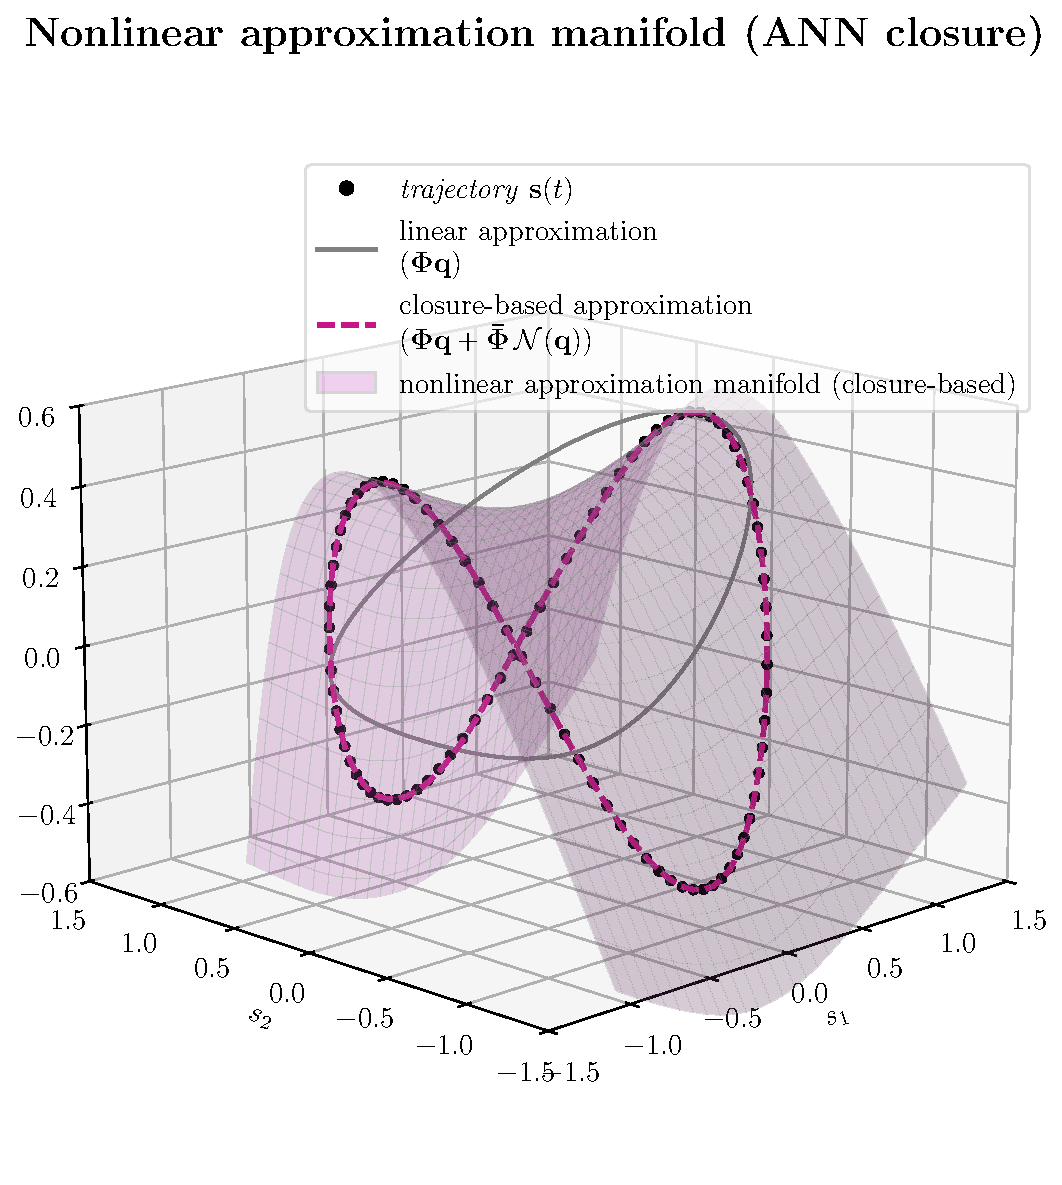
\includegraphics[width=0.6\textwidth]{Figures/nonlinear_closure_manifold_ann.pdf}
  \caption{ANN-based latent-space closure modeling inducing a nonlinear approximation manifold 
for the redundant 3D trajectory. The nonlinear mapping corrects the retained modes to recover 
the full trajectory.}
  \label{fig:toy_ann_manifold}
\end{figure}

\subsection{PROM-ANN with latent-space closure for the model problem}
\label{subsec:latent_ann_model_problem}

The nonlinear latent-space closure framework described in Section~\ref{subsec:latent_ann_formulation} is now tested on the same parametric inviscid Burgers’ problem.
This setup provides an ideal demonstration of how the PROM-ANN architecture can substantially mitigate the Kolmogorov $n$-width barrier by augmenting a minimal set of primary modes with a flexible data-driven correction.

For the offline stage, the full-order snapshots are projected onto a global POD basis and partitioned into retained modes (\(n\)) and discarded modes (\(\bar{n}\)).  
The closure map is constructed using a fully connected feed-forward neural network with five hidden layers and ELU activations, balancing expressiveness with training stability.  
This choice enables the model to learn complex latent relationships efficiently while keeping the regression problem tractable, especially when scaling to high-dimensional industrial meshes.

Figure~\ref{fig:fom_vs_ann_prom_5.19} illustrates the performance of the PROM-ANN at the representative point $\boldsymbol{\mu}_3 = [5.190,\, 0.0260]$ using $n=17$ retained modes and $\bar{n}=79$ discarded modes.
The PROM-ANN approximation significantly improves upon the equivalent global linear POD PROM with the same $n=17$, yielding sharper wavefront resolution and more accurate shock capturing while requiring no local bases or piecewise treatment.
A further comparison with the over-resolved global PROM ($n=96$) shows that the PROM-ANN achieves a competitive level of accuracy with an order-of-magnitude smaller linear subspace.

\begin{figure}[htbp]
    \centering
    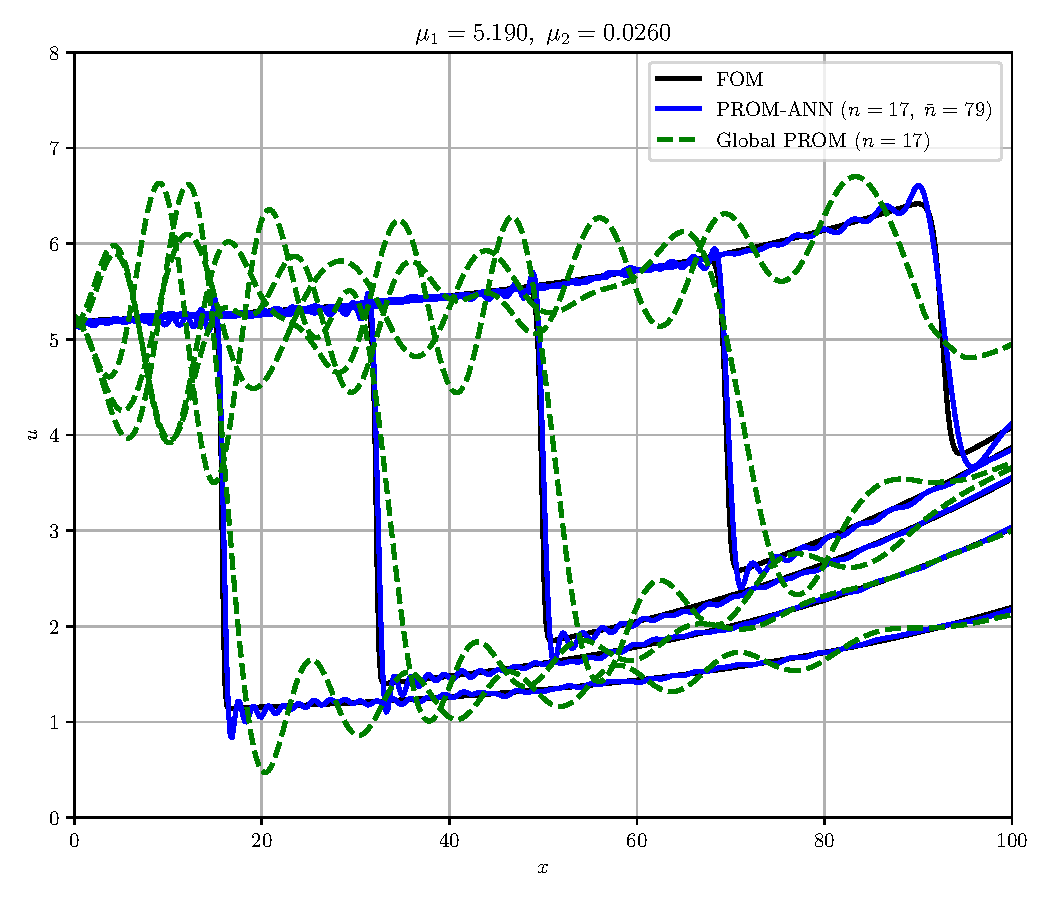
\includegraphics[width=0.49\textwidth]{Figures/fom_vs_ann17_nb79_vs_global17_mu1_5.190_mu2_0.0260.pdf}
    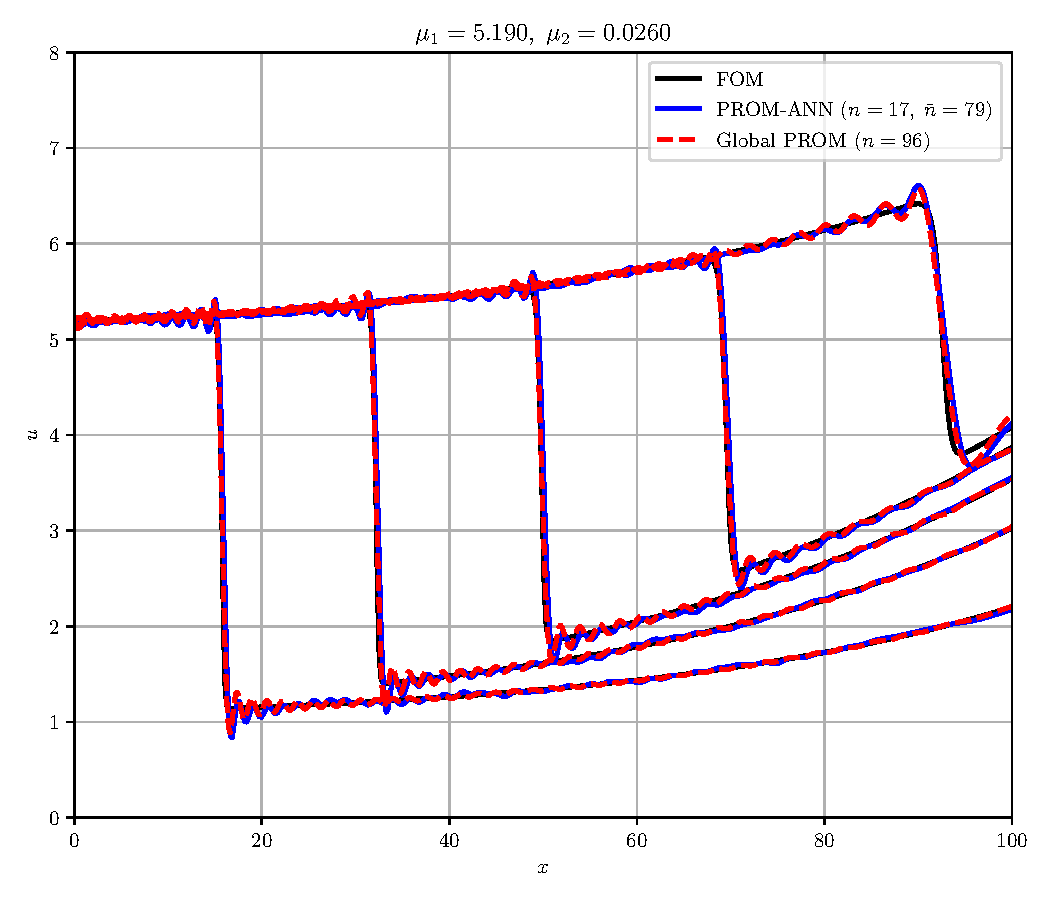
\includegraphics[width=0.49\textwidth]{Figures/fom_vs_ann17_nb79_vs_global96_mu1_5.190_mu2_0.0260.pdf}
    \caption{Comparison of the FOM solution with the PROM-ANN ($n=17$, $\bar{n}=79$) and two global linear POD PROMs ($n=17$ and $n=96$) for $\mu_1 = 5.190$, $\mu_2 = 0.0260$.}
    \label{fig:fom_vs_ann_prom_5.19}
\end{figure}

To further demonstrate the expressive power of the PROM-ANN approach, the retained basis is reduced aggressively to $n=5$, with a corresponding closure space of $\bar{n}=91$.  
Figure~\ref{fig:fom_vs_ann_prom_4.56} shows results at $\boldsymbol{\mu}_2 = [4.560,\, 0.0190]$.  
Despite the drastic dimension reduction, the PROM-ANN preserves a high level of fidelity, dramatically outperforming the global linear PROM with $n=5$ and remaining competitive with the global PROM with $n=96$ modes.

\begin{figure}[htbp]
    \centering
    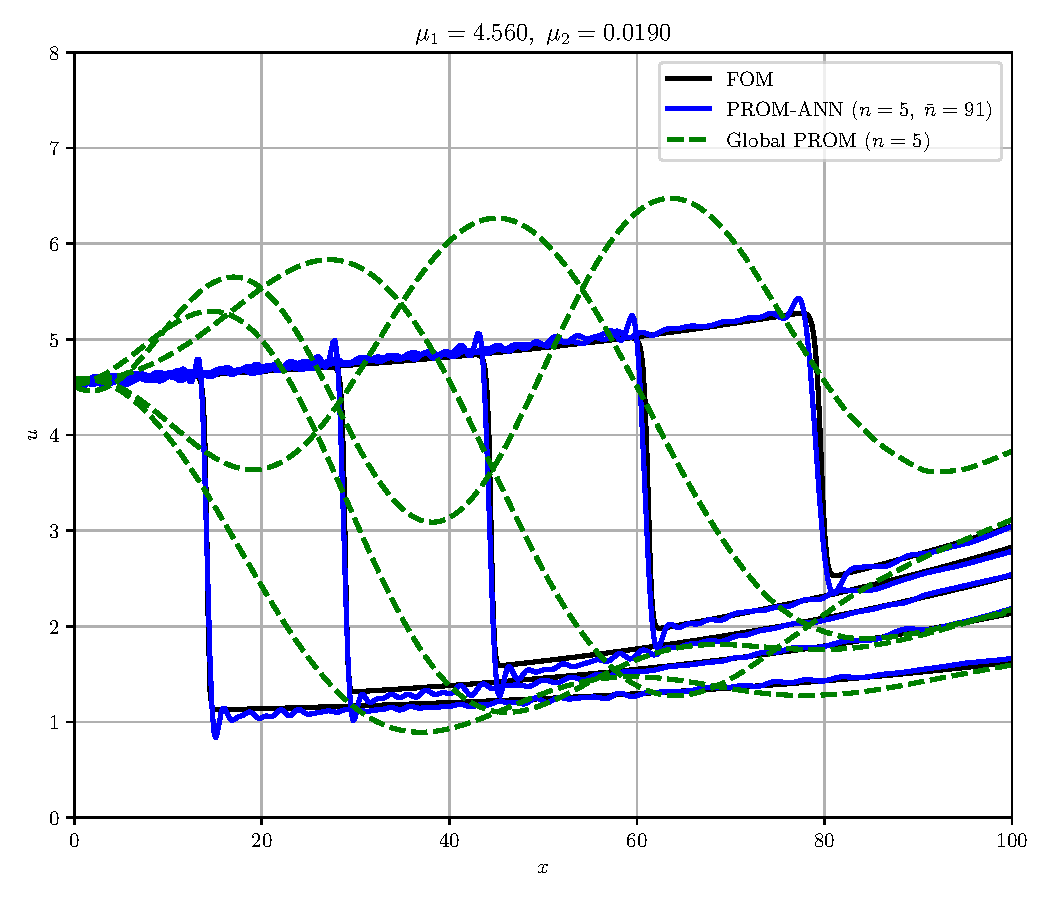
\includegraphics[width=0.49\textwidth]{Figures/fom_vs_ann5_nb91_vs_global5_mu1_4.560_mu2_0.0190.pdf}
    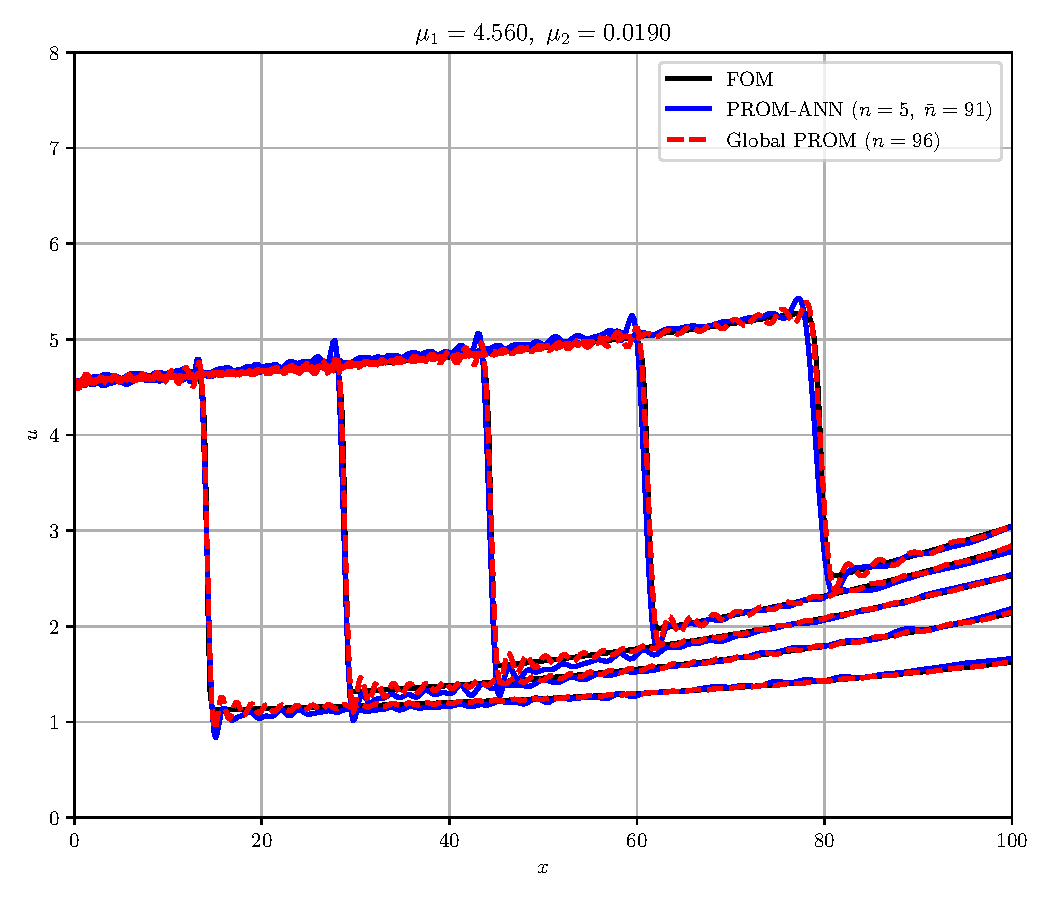
\includegraphics[width=0.49\textwidth]{Figures/fom_vs_ann5_nb91_vs_global96_mu1_4.560_mu2_0.0190.pdf}
    \caption{Comparison of the FOM solution with the PROM-ANN ($n=5$, $\bar{n}=91$) and two global linear POD PROMs ($n=5$ and $n=96$) for $\mu_1 = 4.560$, $\mu_2 = 0.0190$.}
    \label{fig:fom_vs_ann_prom_4.56}
\end{figure}

Table~\ref{tab:prom_ann_error_summary} summarizes the maximum relative $L_2$ errors computed across all three test configurations.
Compared to the best equivalent global linear PROM, the PROM-ANN achieves more than an order-of-magnitude improvement in worst-case error for the aggressively reduced case ($n=5$) and consistently delivers near-optimal accuracy for the moderate basis ($n=17$).

\begin{table}[htbp]
    \centering
    \begin{tabular}{c c c c}
        \toprule
        Computational model & $n$ & $\bar{n}$ & $\mathbb{RE}^{\textbf{max}}_{2, \mathbf{u}}$ (\%) \\
        \midrule
        Global PROM & 17 & - & 13.52 \\
        PROM-ANN & 17 & 79 & 2.40 \\
        \midrule
        Global PROM & 5 & - & 21.23 \\
        PROM-ANN & 5 & 91 & 2.36 \\
        \midrule
        Global PROM & 96 & - & 1.09 \\
        \bottomrule
    \end{tabular}
    \caption{Relative $L_2$ errors for the PROM-ANN and corresponding global linear PROMs across the three test configurations. Maximum values are shown for each setting.}
    \label{tab:prom_ann_error_summary}
\end{table}


These results highlight how latent-space closure modeling with an ANN can push the limits of linear subspace compression in convection-dominated regimes, providing a robust alternative to piecewise or polynomial manifold extensions.
The selected neural network architecture, while simple, demonstrates that even modest latent closures can deliver substantial gains when integrated into a residual-minimizing projection framework.
This flexibility underscores the PROM-ANN’s promise for scalable industrial applications, especially when combined with hyper-reduction strategies to ensure real-time performance.


\section{Towards improvements and alternatives to nonlinear latent-space closure models: discrete physics-informed training and machine learning regression for closure error modeling}
\label{sec:latent_closure_improvements}

The analyses presented in this chapter highlight both the promise and the current limitations of nonlinear manifold PROMs, particularly latent-space closure models. While the PROM-ANN approach demonstrates significant improvements over traditional linear subspace ROMs, especially in convection-dominated regimes, it still inherits key challenges common to data-driven surrogates: limited interpretability, sensitivity to training data availability, and potential inconsistencies with the physics governing the full-order model.

Addressing these aspects suggests methodological enhancements along two complementary directions: introducing \emph{physics-awareness} into the training process and exploring more \emph{transparent regression strategies} for modeling closure errors.

On one hand, ensuring that the learned nonlinear manifold behaves consistently with the governing equations is essential for robust intrusive PROM deployment. Motivated by this need for residual consistency:
\begin{itemize}
    \item \textbf{Chapter~\ref{chap:article3}} presents a discrete physics-informed training approach that augments the standard snapshot loss with a residual-based loss derived directly from the finite element residual. This hybrid training formulation blends data-driven and physics-informed components, explicitly driving the PROM-ANN manifold to represent not only the solution snapshots but also the residual structure that governs the dynamics. As demonstrated in the associated peer-reviewed study, this strategy improves the alignment between offline training and online residual minimization, paving the way for more reliable nonlinear PROMs for strongly nonlinear problems~\cite{sibuet2025discrete}.
\end{itemize}

On the other hand, the reliance on black-box neural networks for closure modeling often complicates interpretability and error certification, especially in data-sparse scenarios. To address this concern:
\begin{itemize}
    \item \textbf{Chapter~\ref{chap:article4}} investigates alternative latent-space closure models based on \emph{Gaussian Process Regression (PROM-GPR)} and \emph{Radial Basis Function interpolation (PROM-RBF)}. Both methods preserve the latent correction structure established in the PROM-ANN framework but replace the deep network with kernel-based surrogates that offer closed-form expressions, tunable hyperparameters, and, in the case of GPR, predictive uncertainty estimates. These regression-based strategies have proven particularly effective for transport-dominated flows and large-scale CFD models, delivering accuracy comparable to PROM-ANN while dramatically reducing data requirements and enhancing theoretical transparency~\cite{de2025nonlinear}.
\end{itemize}

Collectively, these two research directions---physics-informed training and interpretable regression for latent-space closures---form a critical bridge between the foundational PROM-ANN methodology and its practical extension to industrially relevant problems. The next two chapters consolidate these contributions, providing full mathematical derivations, detailed implementation workflows, and extensive validation studies that demonstrate the effectiveness of these advanced nonlinear PROMs.



% \clearpage

% \begin{tabbing}
% \hspace{4cm} \= \kill
% $N$ \> Number of full-order DoFs \\
% $n$ \> Number of retained modes (primary coordinates) \\
% $\bar{n}$ \> Number of discarded modes (closure coordinates) \\
% $N_s$ \> Total number of snapshots available \\
% $N_{\text{train}}$ \> Number of training snapshots for closure model \\
% $N_{\text{local}}$ \> Number of local clusters (piecewise-linear) \\
% $P$ \> Number of parameter samples \\
% $N_t$ \> Number of time steps per parameter \\
% $k$ \> Dimension of symmetric quadratic vector, $k = n(n+1)/2$ \\

% $\mathbf{u}$ \> Full-order state vector \\
% $\tilde{\mathbf{u}}$ \> ROM-reconstructed solution \\
% $\mathbf{u}_{\text{ref}}$ \> Reference state (mean or steady solution) \\
% $\mathbf{q}$ \> Retained reduced coordinates \\
% $\bar{\mathbf{q}}$ \> Latent closure coordinates \\
% $\mathbf{q}_c$ \> Local reduced coordinates (cluster $c$) \\
% $\mathbf{q}_g$ \> Global reduced coordinates for clustering \\
% $\mathbf{c}_c$ \> Cluster centroid \\
% $\delta_{\text{overlap}}$ \> Overlap threshold for clusters \\

% $\boldsymbol{\Phi}$ \> Retained POD basis matrix \\
% $\overline{\boldsymbol{\Phi}}$ \> Discarded POD basis \\
% $\boldsymbol{\Phi}_{\text{tot}}$ \> Total basis before partitioning \\
% $\boldsymbol{\Phi}_c$ \> Local POD basis (cluster $c$) \\
% $\mathbf{H}_s$ \> Quadratic manifold tensor (symmetric) \\
% $\mathbf{Q}_s(\mathbf{q})$ \> Symmetric quadratic monomial vector \\

% $D_u$ \> Nonlinear decoder mapping reduced $\to$ full \\
% $E_u$ \> Encoder mapping full $\to$ reduced \\
% $\mathcal{N}$ \> Nonlinear latent closure map (e.g., ANN, GPR) \\

% $\mathbf{R}$ \> Full residual vector \\
% $\mathbf{J}$ \> Full residual Jacobian \\
% $E_r$ \> Residual encoder for projection \\
% $\mathbf{r}$ \> Reduced residual vector \\
% $\mathbf{G}$ \> Weighting matrix for residual norm \\
% $\epsilon$ \> POD truncation tolerance (global) \\
% $\epsilon_{\text{tol}}$ \> POD truncation tolerance (local) \\
% $\alpha$ \> Tikhonov regularization for QPROM \\

% $\mathbf{S}$ \> Snapshot matrix \\
% $\widetilde{\mathcal{E}}$ \> Reduced mesh / element subset (hyper-reduction) \\
% $\xi_e$ \> Cubature weight for element $e$ \\

% PROM \> Projection-based Reduced Order Model \\
% PROM-ANN \> PROM with ANN latent closure \\
% PROM-GPR \> PROM with GPR latent closure \\
% PROM-RBF \> PROM with RBF latent closure \\
% QPROM \> Quadratic PROM \\
% POD \> Proper Orthogonal Decomposition \\
% LSPG \> Least-Squares Petrov--Galerkin \\
% ECSW \> Energy-Conserving Sampling and Weighting \\
% ECM \> Empirical Cubature Method \\
% PINN \> Physics-Informed Neural Network \\
% \textbf{Discrete PINN} \> Residual-based physics-informed training \\
% Kolmogorov $n$-width \> Best possible linear subspace error measure \\
% $\mathbb{RE}^{\textbf{max}}_{2, \mathbf{u}}$ \> Max relative $L_2$ error (solution) \\
% $\otimes$ \> Kronecker product operator \\
% \end{tabbing}





